\chapter{}\label{chap4}
\addtocontents{toc}{\bigskip}
\addtocontents{toc}{\protect\contentsline{chapter}{\protect \centerline{Chapter \numberline{\thechapter}}}{}}  
\addtocontents{toc}{\medskip}  

\heading{Honours and Awards}
\addtocontents{toc}{\protect\contentsline{section}{Honours and Awards}{\thepage}}
\smallskip

\lhead[{\it\fontsize{9pt}{9pt}\selectfont\thepage}]{\it{\fontsize{9pt}{11pt}\selectfont Honours and Awards}}

\index{Raman, Chandrasekhara Venkata!Awards/Distinctions|(}

\noindent
The awards and honours that Raman received during his lifetime were numerous. Among the earliest, his election in 1924 as a Fellow of the Royal Society, London, was significant both for his scientific career and his public image.

In September 1925, just six months after his return from America, Raman proceeded to Leningrad and Moscow to represent the Calcutta University at the bi-centenary of the Russian Academy of Sciences. He was welcomed with great enthusiasm at the centenary functions and later toured extensively, visiting the Caucusus region, Georgia and the Caspian shores. Returning to Leningrad, he visited Germany {\em via} the Baltic and later saw the lakes of Italy before returning to India.

Raman was knighted in June 1929. He was awarded the Matteucci Medal by the Societa Italiana della Scienza of Rome in 1928. In 1930, the Royal Society of London presented him the Hughes Medal for his distinguished work on optics. During the award-giving ceremony, Lord Rutherford read the following citation:
\begin{quote}
{\fontsize{10pt}{12pt}\selectfont
``Sir Venkata Raman is one of the leading authorities in Optics, in particular on the phenomenon of the scattering of light. In this connection. about three years ago, he discovered that the light's colour could be changed by scattering. This had been predicted some time before, but in spite of search, the change had not been found. The\break RAMAN EFFECT must rank among the best three or four discoveries in Experimental Physics in the last decade. It has proved, and will prove, an instrument of great power in the study of the theory of solids. In addition to important contributions in many fields of knowledge, he has developed an active school of research in Physical Science in the University of Calcutta.''}\relax
\end{quote}

In 1942, the Franklin Institute of Philadelphia awarded him the Franklin Medal. The citation on that occasion said, amongst other things, that the award to Sir C.V. Raman was in recognition of his many brilliant contributions to Physical Science and of his leadership in the renaissance of scientific work and scientific education that has occurred in India. The Soviet Union honoured him with the International Lenin Peace Prize in 1957.

Several Indian universities, amongst them the universities of Calcutta, Bombay. Madras, Benares, Dacca (at that time in India), Allahabad, Patna, Lucknow, Osmania, Mysore, Delhi, Kanpur and Sri Venkateswara, conferred Honorary Doctorates on him. Amongst the universities outside India, mention may be made of the University of Freiburg which conferred on him the Hon. Ph.D. degree and the University of Glasgow which conferred the Hon. LL.D. in 1930. He also received the degree of Hon. Sc.D. of the University of Paris in 1932.

He was an Honorary Member of the Deutsche Akademie of Munich, of the Zurich Physical Society, the Royal Philosophical Society of Glasgow, the Royal Irish Academy and of the Hungarian Academy of Sciences. He was an Honorary Member of Indian Science Congress Association as well as of several other Indian science organisations. He was General President of the Indian Science Congress in 1929 and was President of the Indian Academy of Sciences from its foundation in 1934 till his death. He was a Foreign Associate of the Academy of Sciences, Paris, and a Foreign Member of the Academy of Sciences of the U.S.S.R. He was an Honorary Fellow of the Optical Society of America and the Mineralogical Society of America; an Honorary Member of the Academy of the Socialist Republic of Rumania and of the Catgut Acoustical Society of America; and a Member of the Czechoslovak Academy of Sciences. In 1961, Pope John appointed him a member of the Pontifical Academy of Sciences.

During the Indian freedom struggle, and towards the end of British rule in India, most persons who had been knighted gave up their titles in protest against the British suppression of the freedom movement. Raman did not follow suit. His argument was that he did not get the honour for political reasons or through influence; it was given to him for his scientific achievements and there was no need for him to give it back. After India became independent, the British-conferred titles and honours had no significance. But Raman was always referred to as Sir C.V. Raman.

Amongst the many Indian distinctions he received, special mention must be made of the title {\em Rajasabha-Bhushana} conferred by the Maharajah of Mysore in 1935. This title, when literally translated, would read as `The Jewel of the King's Court'. In 1954, the Government of India instituted the title of {\em Bharat Ratna} (Jewel of India), the highest honour of the land, and conferred it on Raman. He is the only scientist to have been thus honoured up to the date of publication of this book.

During my stay at the Raman Institute,\index{Raman Research Institute} Raman went abroad twice. Once, I think it was in 1956, he was invited to the Lindau
Conference of Nobel Prizemen in Physics, at Lake Constance in Germany. After the conference, Raman went to a few places in Germany. Overall he enjoyed the trip very much. In 1958 he went to Russia to receive the International Lenin Peace Prize.
 This time Lady Raman went with him. At some point, Radhakrishnan,\index{Radhakrishnan, V.} his younger son, joined them and the three travelled together. Raman was away for over a month and he asked me to take care of the affairs of the Institute during that period and deal with all matters including correspondence.
\index{Raman, Chandrasekhara Venkata!Awards/Distinctions|)}

\medskip
\heading{Raman's wide interests}
\addtocontents{toc}{\protect\contentsline{section}{Raman's wide interests}{\thepage}}
\smallskip

\index{Raman, Chandrasekhara Venkata!Traits/Interests}

\lhead[{\it\fontsize{9pt}{9pt}\selectfont\thepage}]{\it{\fontsize{9pt}{11pt}\selectfont Raman's wide interests}}

\noindent
Raman was keenly interested in geology. His knowledge of rocks and rock-forming minerals would surprise even a seasoned \hbox{geologist}. He had in his museum a lovely collection of different types of granites, all of them polished to expose their structure, colour and constituent minerals. Likewise, he had specimens of limestone from all over the world. Several of these had been polished to reveal their colours and patterns. He very proudly used to show visitors polished Carrara marble slabs from Italy and Rentichintla limestone from Andhra Pradesh, India. He had specimens representing sedimentary rocks, slates and sandstone. He could give a learned talk on rock-forming minerals, fossils and the age of rocks.

L. Rama Rao,\index{Rama Rao, L.} a well-known professor of geology at the University of Mysore and a paleontologist, speaks of Raman so: ``Any geologist who had opportunities of meeting C.V. Raman and talking to him about recent developments in any aspect of geology --- as for instance, micropaleontology, which is so far removed from physics --- was soon struck by his amazing capacity to follow with clear insight all that you said and he would soon follow up by putting a number of questions of a fundamental character in the field, which were most thought-provoking and immediately opened out an altogether new outlook in your approach.''

A couple of years before his death, he spent a lot of time studying the geography and the geology of the Krishna Valley (in Andhra Pradesh, India) and the rivers in the region. It was known that at one time this had been an active diamond-mining area and Raman believed that there might still be more diamonds to be mined here. He wrote:
\begin{quote}
{\fontsize{10pt}{12pt}\selectfont
``The river Krishna and its principal tributary, the Tungabhadra, flowing respectively in south-easterly and easterly directions, enter the area shown in the geological maps as the Kurnool formations. Further on, they meet and join up near a place known appropriately as Sangameswaram. The united stream then flows eastwards through the area known geologically as the Cuddapah formations. The actual course of the river in these formations is very tortuous. The stream exhibits a conspicuous double bend in the vicinity of the famous shrine of Srisailam. Further on, it turns sharply northwards and its path lies outside the Cuddapah formations for a short length. But the river soon returns to the area of those formations and follows a course roughly parallel to their crescent-shaped outline. Towards the end of its course in the area, it curves round and then meets obstacles to its flow in the form of hills of considerable height and extension. As a result, the river takes a north-easterly direction in the endeavour to by-pass these obstacle and finds a gap through which the waters can flow again southwards. After passing through this gap, the Krishna flows almost due south. It then widens out as it approaches Vijayawada and, passing through another gap between high hills, flows down into the alluvial plains beyond and then to the sea.

The distance between Sangameswaram and Vijayawada by a strai\-ght flight is 178 miles. But measured along the actual path of the river it is no less than 276 miles, the difference arising from the several deviations from a straight path already mentioned. In cutting its way through the Amrabad plateau, composed of rocks of the Cuddapah system, the river passes through a great gorge about one hundred miles long.

The three rivers Godavari, Krishna and Pennar have built up in the course of ages an extensive coastal area of deposited material extending all the way from Kakinada to Nellore. This area, which is shown in the geological maps as a recent formation, exhibits a curious feature in the shape of a tongue with lateral extensions protruding towards the interior behind Vijayawada and with the river Krishna flowing through it. This feature has evidently resulted as a consequence of the flow of the Krishna towards the sea being arrested by the presence of high ground in the shape of rock formations of the Khondalite series. It is in the material thus deposited by the river before it passes Vijayawada that the diamonds carried down by it were sought for and found in past years.

The first volume of the {\em Journal of the Hyderabad Geological Survey}\index{Journal of the Hyderabad Geological Survey@\textit{Journal of the Hyderabad Geological Survey}} published in the year 1929 contains a compilation of all available information on the ancient diamond mines in the area. The maps appearing in this publication indicate the locations not far from the present course of the Krishna river where the diamonds were taken out. All of them were on the northern side of the river, namely Partial, Atkur, Munnaluru, Mogaluru, Koduvatkallu and Ustapalli, with one very significant exception, namely, Kollur. This last was on the right bank of the river where it takes a sharp turn to the north-east by reason of the presence of a range of hills blocking its flow eastwards. Kollur appears to have been a highly productive locality. It was visited by Tavernier who described the surface workings and stated that some 60,000 people were engaged in the mining operations at the time of his visit.

An intensive and prolonged exploration of any particular locality for diamonds might be expected to result in its ceasing to be productive, sooner or later. This is indeed the actual situation, and the fabulous wealth these mines produced is now only a memory. It is of course possible that several less promising locations were left unexplored, and it is also possible that methods of mining which go down to deeper levels might produce results. An inspection of the maps suggests that the course of the river Krishna above Vijayawada has shifted progressively southwards as the result of the deposition of the material which it brought down, and hence the exploration of areas further removed from its present course, and especially of the areas silted over by the streams flowing into it laterally, might conceivably prove to be profitable. But the chief interest attaching to the subject of the diamonds found in the past in the Krishna valley is in the problem of locating the original source of diamonds and exploiting these original sources to the fullest practicable extent.

The long and tortuous course pursued by the river between Sanga\-meswaram and Vijayawada lies for the most part in what are recognised geologically as the upper Cuddapah formations, and only a small part of the same lies within the formations of
lesser age known as the Kurnools. The actual facts of the case suggest that the diamonds deposited in the lower reaches of the river were a part (and naturally only a very small part) of the material scooped out by the flood waters from the floor and walls of the gorges excavated by them and deposited where the flow was arrested. Whether this action was confined to any particular stretch or stretches of the length of the river or whether it extended over the whole or a greater part of its entire course can only be surmised and must await determination by a careful examination of the exposed areas of the river gorges.

It should be emphasised that the Krishna valley lies much further north than the areas bounded on the west by Lattavaram and Guntakal and on the east by Dhone and Gooty and including especially the well-known locality of Vajrakarur, where there were diamond workings in the sixteenth and seventeenth centuries. The geological maps show that the areas mentioned lie outside the Cuddapah formations, and there is therefore no reason for assuming that the circumstances which led to diamonds being found in these areas at or near the surface of the earth have any bearing on the problem of the original source of the diamonds found in the Krishna Valley. Further, in view of the great age of the Cuddapah formations and the absence of any evidence of volcanic activity in the regions traversed by the Krishna river, there is nothing to suggest that the diamonds in the valley were thrown up and made accessible to erosion by the flow of the river by any such activity in the ages subsequent to the laying down of those formations.

The whole purpose of this article is to indicate that the history of diamonds in the Krishna valley need not be treated as a closed chapter having only a historic interest and that, on the other hand, it may well prove to be a subject of practical importance at the present time if pursued vigorously but with the necessary circumspection.''}\relax
\end{quote}

It is unbelievable that a physicist could have written so candidly and knowledgeably about the geology of a particular region of India!

The lectures which Raman delivered before he wrote this article were received with great interest in Andhra State and it was evident to many who listened to him that he had worked on the subject with great concentration and with deep personal involvement. It is a typical illustration of the intensely devoted manner with which he always tackled whatever subject he chose to study. He was never content with a superficial examination, but always raised doubts in regard to basic assumptions which others did not dare question.

\index{Raman, Chandrasekhara Venkata!Traits/Interests|(}
Raman had a lively interest in meteorology and during the Indian Academy of Sciences' annual meetings he organised many symposia and lectures on various aspects of meteorology. I remember very well the symposium on the ``Physics of Thunderstorms'' that was held during the Academy's Annual Session in Delhi in December 1951. The so-called ``nor'westers'', the thunderstorms that lash the coastal Bengal area, was one of the interesting topics discussed. Raman took a lively interest in the lectures and asked several penetrating questions to obtain a deeper understanding of the atmospheric physics behind thunderstorms.

In the Annual Sessions held in Waltair in December 1956, ``Jet Streams in Upper Air'' was the subject of a talk given by Dr. C. Ramaswamy,\index{Ramaswamy, C.} Raman's younger brother. I remember this talk very well and can still picture Ramaswamy on the dais. He always felt nervous giving a talk before Raman, although he was a fine speaker once he overcame his initial fright. Raman evinced a keen interest in the lecture and asked many questions. He absorbed the account given by Ramaswamy and, almost a decade later, wrote two scientific papers about the origin of jet streams and the general circulation of the atmosphere. Many of the concepts discussed by Raman were well-known, but he brought them all together to offer a simple explanation of the mean westerly jet streams in the upper troposphere and the zonal winds.

What impresses the reader about these papers is his remarkable freshness and simplicity of approach. For instance, he starts with the simple concept of the rotating earth and ends with the most important results in modern meteorology, all in a seven-page paper. Raman wrote these papers on meteorology when he was 80 years of age! He chose ``Weather and Atmospheric Circulation'' as his lecture topic for the Gandhi Memorial Lecture delivered on October 2, 1967; it was later published as an article titled ``Zonal Winds and Jet Streams in the Atmosphere'' in the issue of {\em Current Science}\index{Current Science@\textit{Current Science}} dated November 20, 1967. It was also the theme of his presidential address at the Annual Session of the Indian Academy of Sciences\index{Indian Academy of Sciences} held at Madras on December 19, 1967.


Raman had the unique capacity to examine a problem {\em de novo} in a fundamental way. He approached meteorology as a classical physicist and often made brilliant suggestions. His students filled the Indian Meteorology Department and several of them acquired international reputation as meteorologists. On the lighter side of meteorology and meteorologists, Raman used to remark, ``Meteorology has something common with astrology, for I cannot find a meteorologist who can predict the weather correctly''. This used to evoke loud laughter from the audience, to the chagrin of some of the meteorologists present in the assembly. The person who was particularly sensitive to such remarks was Raman's brother Ramaswamy, who used to defend the profession and the science whenever Raman was beyond the range of hearing. But seasoned meteorologists like K.R. Ramanathan\index{Ramanathan, K.R.} and L.A. Ramdas\index{Ramdas, L.A.} enjoyed the joke with as much relish as Raman intended it to be.

Raman's deep interest in astronomy goes back to his early days. When he visited the California Institute of Technology,\index{California Institute of Technology} Pasadena, in 1924 as a visiting professor he had occasion to spend some time at the Mount Wilson Observatory, which was then
at its peak. Apparently he spent a couple of nights in the mountains taking in the heavenly sights at night and exploring the surroundings during the day. The great l00-inch telescope had gone into operation and in the hands of Hubble\index{Hubble} had yielded some spectacular results, revising Man's concepts of distances in the universe. Raman too viewed the distant stars and gaseous nebulosities through this telescope and the experience stayed fresh in his memory, inspiring his vision of astronomy.

\vskip .1cm

Raman used to often talk about the 200-inch telescope at Mount Palomar with wonder and amazement, saying what a technological marvel it was, scanning the sky with the precision of a Swiss watch. Mount Palomar dominated astronomical research for several decades and its telescope still remains the most powerful optical telescope in the world (see Raman's Convocation
Address later in this chapter).

\vskip .1cm

Raman had a strong desire to install a telescope in the dome of the Spectroscopy Laboratory at the Raman Research Institute,\index{Raman Research Institute} but he never got around to it. He had acquired a few large diameter (one foot or so) reflecting mirrors from one of his friends, H.P. Waran (Parameswaran),\index{Parameswaran, H. (H.P. Waran)} and had dreamed of astronomy with them. He used to talk to Padmanabhan\index{Padmanabhan, J.} about making larger diameter reflecting mirrors for a telescope and would ask if he could grind one of large diameter. Padmanabhan the optimist would shake his head in the affirmative. Raman had a great appreciation of the science and technology of optics and
believed that progress in astronomical science in a country depended on the existence in it of skilled opticians who could
grind, polish and figure great lenses and mirrors to the most exacting requirements.

Raman had filled the Raman Institute grounds with spectacular flowering trees, shrubs and lovely roses. All the best roses that the Bangalore nurseries could supply were planted in his rose garden under his supervision and he would admire them like a child with a new toy. He knew the botanical names of most of the trees and shrubs in the grounds of the Institute and had them planted carefully to maximise the effect of their floral display. He would go around his garden twice a day, to enjoy it, to relax in it and to think of Science. Many a time he would discuss physics with his research students, while taking a stroll in the grounds. Almost every evening, weather permitting, he would go to Cubbon Park for a walk and on several occasions I accompanied him. It was a delight to walk with him, for he kept constantly talking about Science, Nature and other topics uppermost in his mind. He would look at the trees and admire their foliage and flowers. 
\index{Raman, Chandrasekhara Venkata!Traits/Interests|)}

Recalling an encounter with Raman in Cubbon Park, Ramakrishna, formerly a professor in the Electrical Communications department, says, ``Dr. Dhawan\index{Dhawan} and I were walking in Cubbon Park and we saw Prof. Raman searching for something under a lamp post in the dusk. We asked him if we could be of any help and he told us to pick up some of the wings of the insects that come in thousands to a bright light on a suicidal mission, after a heavy shower in the summer months, and lose their wings. We did not have the courage to ask why he wanted them, but respectfully collected a matchbox-full of wings and took it to him. ``Now you can come with me,'' he told us and took us near a mercury vapour lamp on the roadside and held a wing against the light, and, lo and behold, the beautiful diffraction colours from the skeletal structure of the wings appeared in front. Only a naturalist like Raman can see how science permeates all life''.

Sometimes he would pick up fallen seeds and admire their shapes, colours and polish. At times he would fill his pockets with them for a more thorough look at them in the Institute. Lady Raman\index{Raman, Chandrasekhara Venkata!Raman, Lokasundari} would often find strange-looking seeds in his coat pockets and wonder about them. When he reached a wide open space he would look at the stars and point out their names and character.

\vskip .1cm

He would not miss the annual Horticultural Shows in the Lalbagh gardens, a lovely botanical garden near the south Kempegowda tower in Bangalore. Majestic trees of all sorts, rows of flowering trees, flower beds and a glass house are some of the features of this lovely garden. An admirer of Raman who happened to go to the flower show one year remembers, ``The crowd had melted away. One lone figure was standing amidst the flowers with a magnifying glass in one hand and a beautiful Begonia in the other. He was studying the colour pattern through the glass. When I and some friends approached him, he looked at us. There was a far-away, dreamy look in his eyes which showed that his curious intellect had grappled with the colour scheme of the flower, which baffled him. Slowly he came back to earth and talked to us about the new research on which he was engaged''.

\vskip .1cm

Raman\index{Raman, Chandrasekhara Venkata!Traits/Interests} would run into everyone at the Institute at least once during the day to discuss work or exchange a few words. It was not the custom, however, for us to exchange any formal greetings. Many a time on his birthday we wanted to wish him, but none of us did so. Perhaps we felt that being insiders it was not proper for us to do so; perhaps it was the age difference which prevented us from communicating our sentiments. I forget the exact year. It must have been one year in the mid-Fifties when we all decided that we would wish him on his birthday. We got the Institute gardener to make a rose bouquet and I was chosen as the person to present the bouquet to Raman. I accepted the assignment on one condition, that the others would follow me. We all stood in the veranda in front of Raman's room and when he came out I promptly stuck the rose bouquet in his hand and all of us said, ``We greet you on your birthday''. Raman was taken aback for a moment by this act of ours, but was deeply moved. In those days he would not show any emotion outwardly. He took a sniff at the roses and said, ``I say, these are lovely roses, where did you get them? I suppose they are not from my own garden''. We could not lie about the roses and admitted that they were from the Institute garden. Then he said, ``You should have left them on the plants. They would have looked more gorgeous there than in the bouquet. Anyhow, I thank you all''. That was our first and last attempt to formally wish him.

\vskip .1cm

Raman was fascinated by the Alps and the Alpine scenery. He had seen it from different points. Once he told me, ``If ever you go to Europe, don't fail to go to Innsbruck and take a look at the mountains. This is one of the most spectacular sights''. I did go to Innsbruck some ten years later and Raman's words rang in my ears when I saw the spectacular scenery before me. During his Calcutta days, Raman used to go to Darjeeling for vacations, and he would always afterwards talk about the sunrise, sunsets and the majestic snow-covered peaks that could be seen from there. Mountains, lakes, forests, he loved them all and drank deeply of Nature whenever he had the opportunity. His absorption in Nature and Science could never be separated. He derived scientific inspiration from Nature and natural phenomena. He was a modern man in his scientific outlook, but was not distracted by mundane modernism.

For\index{Raman, Chandrasekhara Venkata!Traits/Interests} instance, he would never go to a movie for entertainment. Only once have I seen him going to a cinema house and that was to see a short documentary on the Raman Research Institute that the government films division had made. He took Padmanabhan\index{Padmanabhan, J.} and myself along with him to a movie house in South Parade in the Cantonment section of Bangalore to see this film. The manager of the movie house saw Raman coming and received us. Raman insisted that he would pay the admission charge and handed over ten rupees or so for three seats in the box section. The movie running on that day was {\em Anna and the King of Siam}. The documentaries are usually shown first in Indian cinema halls and we watched the short presentation on the Raman Research Institute\index{Raman Research Institute} in which Raman figured prominently. Raman was quite satisfied with the production and exchanged some comments with us. We then got up thinking that he would not like to sit and watch the movie. But he said, ``I say, let us stay for awhile and see what this cinema is all about. After all, we have paid for it''. We sat for another ten minutes, watching Yul Brunner as the King of Siam. After a little while, Raman became restless and said, ``Let us go. What is all this nonsense that they portray the King of Siam as a bald-headed savage. I don't like all this''. We got up, left the cinema hall and drove home. 

Clouds were another favourite lecture topic with Raman. Cloud patterns in the sky and the brilliant colours they displayed
at sunset fascinated him. He was never tired of looking at the sky and sharing his excitement with anyone around. I once accompanied him and Lady Raman\index{Raman, Chandrasekhara Venkata!Raman, Lokasundari} to the Air Force Officers Club in Jalahalli, a suburb of Bangalore, where Raman had been invited
to give an after-dinner speech. He spoke about clouds! It was a fascinating lecture in which he explained how clouds form and how they assume various shapes. He spoke about cumulus and cumulo-nimbus, stratus and nimbo-stratus and iridescent clouds. He explained how the beautiful diffraction haloes sometimes seen around the moon were caused by ice crystals at very high altitudes. The lecture was a thrilling experience and Raman was enthusiastically applauded for it. He was in great spirits that evening.

The Raman Research Institute museum possessed a collection of stuffed birds, beetles, shells of all kinds and other marine life. He had chosen these specimens mostly for their colour, or for the interesting structures they often exhibited. Among the birds were blue jays, golden orioles, pheasants. The beetles were either iridescent or exhibited some interesting pattern of colour. He derived tremendous pleasure looking at them periodically and talking to visitors about them.

He once brought from a taxidermist in Calcutta two beautiful stuffed Himalayan pheasants for the museum. We left these pheasants in an open almirah and forgot to lock the door of the room. As ill-luck would have it, two mongrels got wind of the
stuffed birds. They gained entry into the room at night and destroyed one of the pheasants beyond recognition. The next morning, when we came in and saw the spectacle, it was a shock. We knew that Professor would get very upset with us for not locking the room, so something had to be done to cover up the catastrophe. We quickly ordered the servants to clean up the place and bury the remnants of the pheasants in a far off place.

When Raman came, he went straight to the museum room. Not finding one of the pheasants, he wanted to know what had happened to it. We had decided to maintain that there had been only one pheasant. Professor repeatedly said that he had definitely bought two and kept scratching his head wondering how one could have disappeared. Since we continued to maintain that there had been only one pheasant, he finally convinced himself that although he had paid for two, only one specimen had actually been sent to Bangalore. Then he went for a walk in the gardens, satisfied with his reasoning.

Twenty minutes or so later, he returned with a feather in his hand; it was obviously the feather of the same pheasant which the mongrels had torn to pieces. The man who had taken the remnants must have dropped a feather on the way. It was difficult to maintain our cover-up story, but we managed to convince Professor that some other bird must have dropped a feather on its flight. Raman must have wondered about it all, but did not ask any further questions. We felt very bad about having hidden the truth from him. But since we had just joined, we did not want to run the risk of being sent away by revealing what had actually happened.

\medskip
\heading{The Raman spirit and his traits}
\addtocontents{toc}{\protect\contentsline{section}{The Raman spirit and his traits}{\thepage}}
\smallskip

\index{Raman, Chandrasekhara Venkata!Traits/Interests|(}

\lhead[{\it\fontsize{9pt}{9pt}\selectfont\thepage}]{\it{\fontsize{9pt}{11pt}\selectfont The Raman spirit and his traits}}

\noindent
Raman was an intense person who became engrossed in whatever subject interested him. Whether it was in the field of Science or outside it, he was never content with a superficial examination. When he was in the Financial Civil Service, he paid meticulous attention to his official duties and was lauded by his superiors for his prompt and intelligent way of handling anything connected with them.

There is a story, recalled by a citizen of Nagpur, whose collection of a few hundred-rupee notes was nearly burnt by a fire. The perturbed individual went to the Accountant-General's Office and presented the half-burnt bundle there, but with little hope of receiving any satisfaction. Any other officer would probably have shown him the door, but Raman, who was then in the office of the Accountant-General, took the trouble to scrutinise the notes one by one, using a magnifying glass, and then instructed the treasurer to give the petitioner fresh notes. Raman argued that the numbers on the half-burnt notes were visible and it was, therefore, a genuine case. This incident is characteristic of the thoroughness with which Raman tackled all problems he faced. Between 1907 and 1917, the leadership Raman offered and the tremendous enthusiasm he whipped up for scientific research in Calcutta were reflected in his address at the Science Convention for 1917 held in the presence of Sir Asutosh Mookerjee.\index{Mookerjee, Asutosh} He said:
\begin{quote}
{\fontsize{10pt}{12pt}\selectfont
``The ten years, from July 1907 to June 1917, which preceded my joining the University of Calcutta as Palit Professor of Physics, afforded me numerous opportunities for studying, as an impartial and disinterested observer, the efforts made during the period in this University towards fostering higher studies and research in physics. Looking back over these years, one cannot fail to be struck with the genuine progress that has been achieved and with the fact that, today, the Calcutta University\index{Calcutta University} can claim to possess a real School of Physics, the like of which certainly does not exist in any other Indian university, and which, even now, will not compare very unfavourably with those existing in European and American universities. What has impressed me most is the rapidity of the progress, the position now being very different from what it was ten years ago, and this is obviously a most hopeful sign for the future.}\relax

{\fontsize{10pt}{12pt}\selectfont
My own work at Calcutta commenced in 1907 and was made possible by the special facilities put at my disposal by the present Honorary Secretary, Dr. A.L. Sircar,\index{Sircar, Amrit Lal} who had the Laboratory kept open at very unusual hours in order that I might carry on research in the intervals of my duties as an officer of the Indian Finance Department. Gradually others were drawn in to take part in the revived activities of the Association. The success which has attended these efforts is indicated by the fact that during these ten years the Association has issued as its own publications, fourteen special {\em Bulletins}, and three volumes of {\em Proceedings},\index{Proceedings of the Indian Association for Cultivation of Science@\textit{Proceedings of the Indian Association for Cultivation of Science}} besides publishing its Annual Reports. These publications have been warmly received abroad, and the Association is now in exchange relations with about fifty learned societies and institutions in various parts of the world.''}\relax
\end{quote}

Raman went on to add:
\begin{quote}
{\fontsize{10pt}{12pt}\selectfont
``A wide range of subjects is at present attracting the attention of the Calcutta School of Physics. General Physics, Acoustics, Optics, Electromagnetic Theory, Electric discharge, Spectroscopy, X-Rays and Resonance Radiation and Radio-activity have all come in for a share of attention, and this wide range of interest will become even more manifest when our equipment is more complete, and I have had time to take on a large number of research workers and train them. ....Perhaps the most significant tributes to the fact that we have now a real scientific atmosphere at Calcutta are the numerous requests that have been received from teachers and scholars in various parts of India and Burma to be permitted to work in my laboratory and to carry on research.''}\relax
\end{quote}

In the closing section of his report, Raman stressed the need for (i) strengthening the equipment of the Department of Physics of the Calcutta University, (ii) provision of residential accommodation in the premises of the College of Science to enable the professors and staff to devote all their time to work in the laboratory, and (iii) enlargement of the careers open to workers. He concluded his remarkable address with the statement that ``to most men, the knowledge of the degree of recognition that awaits successful work is a stimulus not to be despised''.

His physical energy was as extraordinary as his mental output. An outstanding characteristic of Raman was that, unlike other persons, he seldom relaxed. He was always keyed up to fever pitch by the continuous thrill or excitement that the challenges and the ever-expanding avenues of scientific research provided his mind. He was capable of tremendous concentration on intellectual work, as the following incident will show. Once, in Calcutta, when he was in his office at the Association, drafting a rather tough paper for publication, a Swamiji visited him. He welcomed him courteously, asked him to take a seat and said that as soon as he finished the work he was busy with, he would be glad to spend some time with the Swamiji. Then, for the next couple of hours, he was completely oblivious of the Swamiji. When he completed the task on hand, he suddenly looked up and found the Swamiji still waiting. Raman told him that as he had only five minutes now left before he had to attend another pressing engagement, would the Swamiji be brief. The Swamiji was equal to the occasion. He told Raman that deep concentration was what a spiritual person had to practice. And Raman already possessed this, as was demonstrated by the fact that he had been oblivious of all else for the past two hours while he worked. A donation the Swamiji then requested for a charitable cause was instantaneously given by Raman.

The period between 1920 to 1928 may be said to have been the golden period in the scientific life of Raman. Given the combined control of the Association and the University laboratories, he maintained a hectic schedule. L.A. Ramdas\index{Ramdas, L.A.} has described his activity at this time thus:
\begin{quote}
{\fontsize{10pt}{12pt}\selectfont
``The daily activities at the laboratories of the `Association' usually started by 7 a.m. Having started an experiment, one would go on working until 1 p.m. After a quick lunch, the scholars would be back by 2 p.m. and work on far into the evening and often until 9 or 10 p.m., until the job on hand had reached a satisfactory stage. Working at this furious rate, it is no wonder that many of the pupils could work through five or six major investigations each year. Those who could not cope with such a fast tempo of work would automatically drop off.

By 1920, Prof. Raman had gathered round him an increasing number of extremely bright and capable pupils so that, more and more, he could get his research programme executed rapidly by them. He inspired his scholars to use their own initiative and ingenuity to the fullest extent. He would see what was going on and discuss results at intervals. At any given time, however, he would concentrate his attention on the particular scholar who was then entering the most critical phase of his research. Interpretation of results, fruitful suggestions to carry the investigation several stages further and quick discussion of results already obtained resulted in immediate publication from this effective type of collaboration between the Professor and the pupil. Each of his pupils had his opportunity for such exhilarating collaboration at the developing phase of his investigation. All the time, the pupils enjoyed the fullest freedom to think, work and improvise for themselves. Spoon-feeding of any kind was absolutely taboo. A spirit of perfect understanding and goodwill pervaded the entire `Association', with Ashu Babu, the Assistant Secretary, ever ready to help us with any material or facility that we needed, the scholars themselves helping each other spontaneously.''}\relax
\end{quote}

\vskip -.15cm

Raman maintained this mode of working and dealing with students throughout his career. Anyone who wished to work under Professor Raman as a regular student had to undergo a searching oral examination in which the candidate's knowledge of fundamentals and capacity for original thinking would be severely tested. Although he attached importance to academic records, Raman always made a personal assessment. Once selected, the students felt at ease, for Raman was kind and large-hearted with them. Raman had his own way of developing self-confidence and self-reliance in students. He would treat them as his equals, while discussing scientific matters. It was his habit to go round the laboratory every morning, meeting each student and discussing the progress of his work, often suggesting new ideas. He would give free expression to his joy when a new result was brought to his notice. Nagendra Nath\index{Nath, Nagendra} recalls, ``One day, when I told him that I had found the explanation of the Raman line in diamond, which had been mentioned by him as an outstanding problem in his Nobel address, he asked me what it was. I said that the Raman line was to be attributed to the mutual vibration of the two face-centred lattices composing the diamond lattice. He simply yelled out, ``You are right, you are right,'' and insisted that the research paper should be immediately written up. He was in ecstasy over this work. I found myself elected to the Fellowship of the Indian Academy of Sciences,\index{Indian Academy of Sciences} at the age of 23, without an inkling being given to me by Professor''.

\newpage

To criticism that he was partial to students from Madras University,\index{University of Madras} Raman answered, ``They teach very little physics and hence I get very good raw material to work with''. I don't think the criticism levelled against Raman was fair, for Raman's students came from all over India and he did not practice narrow parochialism. He chose them on the basis of merit and shaped them into scientists who went out to carry on the tradition of research wherever they went and worked in their subsequent career. Throughout his life, he had a very warm corner in his heart for his many pupils and they, in turn, knew they could always turn to him for any help that they needed.

In his public lectures, Raman would often refer to his students by name and talk about their work. All this was a thrilling experience to young students and a powerful incentive for hard work. A unique rapport was, thus, established between him and his students.

\medskip
\heading{Thrill of quick publication}
\addtocontents{toc}{\protect\contentsline{section}{Thrill of quick publication}{\thepage}}
\smallskip

\lhead[{\it\fontsize{9pt}{9pt}\selectfont\thepage}]{\it{\fontsize{9pt}{11pt}\selectfont Thrill of quick publication}}

\noindent
From the very beginning, Raman held the view that scientific results should find prompt publication. He practiced this throughout his life. According to L.A. Ramdas, hardly a week passed in the Association at Calcutta without a detailed paper, and, often, shorter notes, being dispatched to foreign journals or to the Calcutta University Press, which published the {\em Proceedings of the Indian Association for Cultivation of Science}.\index{Proceedings of the Indian Association for Cultivation of Science@\textit{Proceedings of the Indian Association for Cultivation of Science}} He was so very critical in composing and editing scientific papers, whether his own or of his pupils, that often it would get too late to post the paper to the publishers in the ordinary manner. So he would hail a taxi and rush to the General Post Office, pay the late fee and get the paper despatched in the nick of time. After many an adventure of this nature, he would share his joy, over sending away in time an important paper for publication, by treating the anxiously waiting group of pupils to a solid feast of {\em sandesh} and
{\em rasogolla} that he would send for from famed ``Bhim Nag'' of College Street, remembers Ramdas.

By securing such quick publication of the results of the researches carried out by himself and his scholars, Raman never allowed scientists elsewhere to anticipate his results. Invariably, a good scholar would have enough published papers to his credit so that, within a couple of years, and, occasionally, even within a year, he would be in a position to submit his doctoral thesis. 

Raman encouraged his scholars to take up independent positions in scientific departments or in the universities quickly, for his policy was that his laboratory should be a `source', not a `sink' of young scientific talent. These brilliant pupils very soon carried the `Raman tradition' of original research wherever they went and worked in their subsequent careers.

\medskip
\heading{Raman as a teacher}
\addtocontents{toc}{\protect\contentsline{section}{Raman as a teacher}{\thepage}}
\smallskip

\lhead[{\it\fontsize{9pt}{9pt}\selectfont\thepage}]{\it{\fontsize{9pt}{11pt}\selectfont Raman as a teacher}}

\noindent
I quote from L.A. Ramdas's\index{Ramdas, L.A.} article on Raman as a teacher:
\begin{quote}
{\fontsize{10pt}{12pt}\selectfont
``Prof. Raman, as a Palit Professor, had no teaching responsibilities, but he enthusiastically took part in M.Sc. teaching. He held the view that when a leading research worker takes on some special teaching course, he brings to his teaching the freshness of research and the questioning attitude which makes all the difference between dull pedagogy and inspired teaching. To some of us who had joined the M.Sc. course at Calcutta (both myself and the late Dr. K.S. Krishnan\index{Krishnan, K.S.} had joined the M.Sc. course in physics at Calcutta by 1920) Prof. Raman once made the side remark that the best way for him to master or revise any subject in physics was indeed to lecture on it to the M.Sc. classes.

The M.Sc. teaching used to be naturally shared by the various professors and lecturers. Prof. Raman took ``Electricity and
Magnetism'' in the year 1920-21 and ``Physical Optics'' in 1921-22. Both sets of M.Sc. students felt that they were indeed
listening to a type of inspired teaching to which was brought all the original flavour and excitement of the great giants of the past who had built up the subject under treatment. In listening spell-bound to Prof. Raman's lectures in ``Electricity and Magnetism'', covering a series of nearly 30 lectures, we had shared with him much of the excitement and superb thrill that Benjamin Franklin,\index{Franklin, Benjamin} Oersted, Arago,\index{Arago} Gauss,\index{Gauss} Faraday,\index{Faraday} Maxwell,\index{Maxwell} Hertz,\index{Hertz} Lord Kelvin\index{Kelvin} and many others must have felt while they were making their actual discoveries. This was indeed no routine text-book learning, but reliving the actual past history of the subject.

\newpage

Almost regularly, Prof. Raman, with his genius for the subject, his extraordinary eloquence, imagery and fullness of precise expression, used to forget himself as well as the time and used to lecture for far more than the prescribed one hour, while the next lecturer was politely (and perhaps with a sense of relief) retiring from the scene after seeing Prof. Raman still at his lecture! Often he used to take the entire forenoon, for more than two and sometimes even three hours --- such was his tremendous love of teaching. The mathematics was worked through often with his own improvised simplifications and fully illustrated with physical analogies. Any question or point raised by a student would start him off towards uncharted grounds, not touched upon in any textbook. His ready wit and sparkling intellect were a treat to the classes. And after each lecture we used spontaneously to look up original papers and classical treatises like Maxwell's\index{Maxwell} ``Electricity and Magnetism'', J.J. Thomson's\index{Thomson, J.J.} ``Conduction of Electricity'', Faraday's\index{Faraday} ``Experimental Researches'', Lord Rayleigh's\index{Rayleigh, Lord} and Kelvin's\index{Kelvin} ``Collected Papers'' and so forth. The lecture in which he worked out Maxwell's field equations and showed that light waves are only electromagnetic waves and the thrill he communicated to the class are still fresh memories.

In ``Physical Optics'', a topic on which he himself was conducting several investigations at the time, the students were introduced to all the topics coming, as it were, hot from the `Lab', and the lecturer's flair for dipping straight into the great masters like Huygens,\index{Huygens} Fresnel,\index{Fresnel} Mascart, Schuster,\index{Schuster} Wood,\index{Wood, R.W.} Rayleigh, and others of the late 19th and the early 20th centuries, imbued the students with a real love and enthusiasm for what they learned at Prof. Raman's feet, as it were. Whether the subject was ``Thermodynamics,'' or the ``Kinetic Theory of Gases'' or ``Modern Physics'', Prof. Raman's treatment of the topic at hand was original and inspiring and left a permanent impression in the student's mind.

``Now let me record a few reminiscences. As an M.Sc. student having direct and free access to Prof. Raman's own personal library, I was astounded to discover that in each and every text book which he had learned from in his own student's career, there were marginal criticisms or appreciations of the author. There was no book in which every example and question had not been worked out by Raman. Some questions had the side remark ``excellent'', while not a few were \hbox{apostrophised} as ``elementary'' or ``silly''! I had no doubt that Prof. Raman had been a most painstaking student and that the definition of `genius' as the `capacity to take infinite pains' is indeed true.''}\relax
\end{quote}

\begin{figure}[t]
\centering
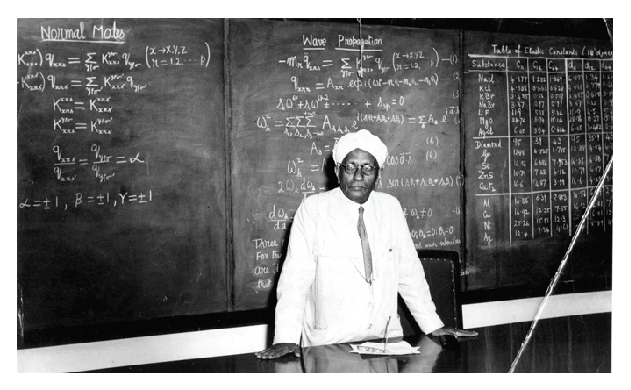
\includegraphics{eps/14.eps}

{\fontsize{10pt}{12pt}\selectfont \em Raman as a teacher}\relax

{\fontsize{10pt}{12pt}\selectfont (Photo Credit : Raman Research Institute)}\relax
\end{figure}

Raman thus fully participated in teaching and inspired his students with his enthusiastic lectures. M.N. Saha,\index{Saha, Meghnad} who later become famous for the ``Ionisation equation'' named after him, and S.N. Bose,\index{Bose, S.N.} discoverer of ``Bose statistics'', were some of the other lecturers at the University College in 1917.

\medskip
\heading{Raman lectures}
\addtocontents{toc}{\protect\contentsline{section}{Raman lectures}{\thepage}}
\smallskip

\lhead[{\it\fontsize{9pt}{9pt}\selectfont\thepage}]{\it{\fontsize{9pt}{11pt}\selectfont Raman lectures}}

\noindent
Raman excelled in public speaking and could give a lecture on, for instance, Egyptian History, off the cuff. His scientific lectures were a treat, for he was a superb entertainer. They were delivered in a high-pitched resonant voice which reached the entire audience, making loud-speakers unnecessary. Rich in imagery and eloquence, and replete with spontaneous jokes, the lectures were given in so popular a style that every listener felt that he understood all the science that the learned lecturer was discussing. Once, he told me that ``the hallmark of a good speaker is that the audience must be under the delusion that they have understood everything that was said by the speaker''. And that is what he used to do, whenever he gave a public lecture --- he would create in the minds of thousands of his listeners, the illusion that they understood everything he spoke about.

Raman's typical way of giving a lecture has been beautifully described by Kashyap:
\begin{quote}
{\fontsize{10pt}{11.7pt}\selectfont
``A tall, turbaned figure, casting those searching and curious eyes almost with child-like fitfulness, would walk directly to the dais, with an occasional turn to the right or left, acknowledging a remark or answering a query by the sponsors of the lecture who were leading him to the dais. Confidence incarnate was the figure and even before he started speaking one got the impression that here was a lecturer who would deliver the goods.


His very presence perhaps cut short the long-winded preambles and welcomes that often mar the beautiful effect of a nice lecture. Prof. Raman meant business and a disapproving look would stop a vagrant introduction. His first words uttered in a characteristically punching manner would set the pace for the lecture.

He spoke of soap bubbles. And, mind you, for some half an hour the evanescent soap bubble that hardly lasts for a couple of seconds blissfully lived!

Raman asked `Have you ever thought of keeping the soap bubble alive for a long time?' An intriguing question --- a question that had never occurred to many. The problem you know, Raman went on to say, is to see that the droplet of water does not collect at the bottom. Then he went on to say how he and other scientists, some in France, managed to keep a soap bubble alive for a few days by subjecting the bubble to an oppositely directed force.

One would never have a dull moment and would not even realise that the lecture was over. To listen to Raman was something more than learning physics. He had the knack of using the most appropriate expressions, which no textbooks could give. He had the habit of tugging the lapels of his coat which was a Raman characteristic. He would invite questions and answer them all with astounding clarity.''}\relax
\end{quote}

He was forthright when he criticised. During the annual meeting of the Indian Academy of Sciences\index{Indian Academy of Sciences} in Baroda in 1958, he interrupted the talk of a high-energy physicist who was filling the blackboard with mathematical equations, and said, ``My dear fellow, please try to explain what you have done in a few sentences. If you cannot do this, it is not worth knowing''.

At the annual meeting of the Academy held at Osmania University,\index{Osmania University} Hyderabad, in the mid-Sixties the then Governor, who was also the Chancellor of the Osmania University, gave a long welcome speech. During the course of the speech, the Governor stressed the importance of scientists stopping ``ivory tower'' research and diverting their attention to problems connected with import substitution, export promotion and defense preparedness. After further advice along these lines to the Fellows of the Academy, the Governor concluded: ``Now, you will hear the learned address of Prof. Raman who is going to speak on the `Physiology of Vision'. You and I will not be able to understand what the learned lecturer is going to say, but as you all know, Prof. Raman is a Nobel Laureate and a great scientist.''

Prof. Raman, well-known for the clarity of his speech and simplicity of his scientific message to a general audience, was
obviously hurt by the Governor's ``Welcome Remarks''. He, however, did not reveal his feelings but went on to deliver a remarkably lucid and clear enunciation of his findings during the year on the ``Physiology of Vision''. Then, before sitting down at the end of the lecture, he turned to the Governor and said, ``Mr. Governor, when I received the Nobel Prize, my illiterate old aunt asked me to explain what exactly I had done to merit such a prize. When I explained to her the finding referred to as the `Raman Effect', she remarked that what I had discovered was so simple that she was surprised that my findings should have merited such a high international prize. I hope, you, Mr. Governor, were able to understand at least some of the things I said''. He then sat down amidst a prolonged, standing ovation.

Raman's lectures were painstakingly prepared and illustrated with colourful slides and diagrams. I often used to prepare these for him and he would ask me to operate the projector, for he could not stand an erring projectionist. I once photographed in colour optical effects exhibited by several gem materials. Colour photography was still an art in those days and not mechanised and automated as at present. Raman took the film with him to Bombay and had it processed. The colour slides turned out to be very good and, he was therefore tremendously happy. He immediately sent an express telegram to me in Bangalore conveying how pleased he was with the outcome. Not only would he always express spontaneously his appreciation and admiration for any good work, but he would also acknowledge in public how so-and-so had done a marvellous job, had discovered something nice or had a good idea.

The excellently lit Raman Institute\index{Raman Research Institute} hall was very well-equi\-pped. It had a fine black ground-glass board covering almost the entire wall on one side. A long, finely-polished teakwood table was positioned in front of the speaker. One hundred plush, cushioned chairs made of teak and upholstered in black velvet were arranged neatly in rows, on an ascending platform. The chairs, wide and with arm-rests were very comfortable. Raman wanted the most comfortable seating possible for the audience in his lecture hall. He used to deliver all his scientific lectures as well as special lectures here.

\vskip .1cm

Every year, in October, he would give what was called the Gandhi Memorial Lecture. The Gandhi Peace Foundation had created a special endowment fund for this lecture. These lectures were well attended, for it was one occasion when the public could listen to Raman. The lectures were free, but tickets were issued on a first-come, first-served basis. Raman used to take a scientific topic on which he was working or he would choose one that he had some interest in and make a masterly presentation of it. On one occasion, he spoke about the {\em Physiology of Vision}, on other occasions he talked\index{Raman, Chandrasekhara Venkata!Papers/Publications/Addresses} about {\em Earthquakes, The Atmosphere, Voice} and {\em Speech and Language}. The last Gandhi Memorial Lecture he gave was on October 2, 1970.

\medskip
\heading{Some reflections on Raman's personality}
\addtocontents{toc}{\protect\contentsline{section}{Some reflections on Raman's personality}{\thepage}}
\smallskip

\lhead[{\it\fontsize{9pt}{9pt}\selectfont\thepage}]{\it{\fontsize{9pt}{11pt}\selectfont Some reflections on Raman's personality}}

\noindent
There are some features of Raman's personality that have been noticed and admired by those who were close to him as well as by those who knew him only at a distance. He was richly endowed with a child-like sense of wonder at the unknown and un-understood facets of Nature and, throughout his life, he was pushed into exploring these aspects. Such being the motivation, he was often, and appropriately, referred to as a Child of Nature, nothing fascinated him more than Nature itself. Subjects like the origin of colours in minerals, birds and butterflies, the blue of the ocean, the sky and other natural phenomena were his primary concern. On the other hand, he could never reconcile himself to the fact that large human resources and material wealth were being put into such programmes as those that dealt with Space and so on, which did not concern themselves with things on earth or with anything of immediate interest to mankind.

\vskip .1cm

His delicate sense of humour, his ability for biting sarcasm when needed and, above all, his love of Nature became very evident whenever Professor Raman wrote or spoke about any subject. On one occasion, while speaking about the countryside and weather, he prefaced his talk with the following remarks:
\begin{quote}
{\fontsize{10pt}{12pt}\selectfont
``To the dweller in the towns, the weather is nothing more than a minor inconvenience which can be minimised by a little forethought in the matter of taking an umbrella instead of a walking stick when going out of the house. I will go so far as to say that the average city dweller is scarely conscious of the weather except when he is reminded of it in some particularly unpleasant fashion. The changing panorama of the skies, the most gorgeous sunrises and sunsets, pass mostly unheeded by him, for, alas, the only landscapes that stretch before his eyes are long rows of tenement houses, and, as for the sky, it is only seen in little patches here and there, not infrequently cut across by great bunches of telephone wires. The only stars that he sees at night are those that shine on the silver screen at the cinema theatre, and as for the sun and the moon, he knows they are there but does not feel called upon to take notice of them more than he can help.''
}\relax
\end{quote}

His own attitudes to certain basic issues of Science and its pro\-gress were often expressed in his public speeches and private conversations. Here is an example of what he thought about discoveries in science:
\begin{quote}
{\fontsize{10pt}{12pt}\selectfont
``It should be mentioned that the reception given at first to even capital discoveries by the outer world is not always one of respectful admiration for the achievement of the discoveries. One of the commonest ways in which the achievement is sought to be minimised by the unthinking or the envious is by attributing it to accident or a stroke of luck akin to the winning of a lottery ticket. Such comments are, of course, deplorable and indeed quite meaningless. The idea that a scientific discovery can be made by accident is ruled out by the fact that the accident, if it is one, never occurs except to the right man. The happy discoverer in Science is invariably a seeker after knowledge and truth, working in a chosen field of his own and inspired in his labours by the hope of finding at least a little grain of something new. The commentators who like to consider discoveries as accidents forget that the most important part of a scientific discovery is the recognition of its true nature by the observer, and this is scarcely possible if he does not possess the requisite capacity or knowledge of the subject. Rarely indeed are any scientific discoveries made except as the result of a carefully thought-out programme of work. They come, if they do come, as the reward of months or years of systematic study and research in a particular branch of knowledge.''}\relax
\end{quote}

One of his favourite comments was about Science being a very particular and difficult mistress. He would say that she would not yield if you wooed her for her wealth; she insisted that you love her for herself and, even then, she would never give herself up completely to anyone but would reveal her secrets only in part and only little by little. As many discerning critics have said, let us not forget, when we discuss and attempt to assess Raman, that he is the greatest contribution India has made for many centuries to systematised human knowledge. We should not fall into the trap of regarding him as {\em just} a successful scientist, like we generally regard other successful scientists or successful businessmen or successful politicians. Men like him are not thrown up every day and, if the rugged contours and the sharp corners of this giant did not compromise with the soft-spoken ways of the successful world, we can only describe the\break phenomenon by stating that ``it is no reproach on Everest that one cannot play golf on it''.

That Raman had to work amidst disappointments, had to struggle and survive many difficult situations before reaching the pinnacle of scientific glory the hard way is not often clear to many. He occasionally used to slip into a reminiscent mood and say that the more he looked back on his career, the more he felt that it had been a long history of frustration, disappointment, struggle and every kind of tribulation. It sounded incredible but true, although some comfort and self-confidence were forthcoming in the same breath, when he used to say, ``There have been a few gleams of success. It was poverty and the poor laboratories that gave me the determination to do the very best that I could''. On one occasion, after reading a glossy biographical note written by one of his associates, Raman remarked that the biography tempted him to picture himself as a prince sitting in a gold chair marching from triumph to triumph, without a tear. While he wished that the picture were true, he knew that in fact it was not so.

In the life of great scientists, there have invariably been periods of distress amidst the joys of scientific successes. Raman's life was no exception. He had to face difficult times both in Calcutta and at the Indian Institute of Science,\index{Indian Institute of Science} Bangalore, causing him severe emotional drain. The difficulties had nothing to do with Science but with the politics of Science of the times.

After the discovery of the Raman Effect in 1928, and following the award of the Nobel Prize in 1930, Raman became a celebrity, his stature in India and abroad growing to new heights. Raman's rise to scientific eminence, power and prestige caused envy in some quarters and Raman had a trying period. The last few years of his stay in Calcutta were by no means happy. Some individuals accused him of not having been fair to young students from Bengal and attributed motives to the manner in which he selected his colleagues and his assistants. Although much of this was a parallel growth alongside his increasing reputation and growing scientific eminence, and was ignored as such by many discerning persons, it nevertheless assumed ugly proportions occasionally. His connections with the Indian Association for Cultivation of Science,\index{The Indian Association for Cultivation of Science} where undoubtedly his best scientific work was done, had to be broken off in an unceremonious manner. He had to defend himself by sharply reacting to public criticism. At one stage, he made a statement that he could have contented himself ``by creating only a Bengali School of physics and not an all India school. But, in that case, I am quite certain that the Nobel Prize in physics would not have come east of Suez''.

One of the leading daily newspapers of Calcutta wrote, in an editorial critical of Raman's methods, that ``a scientist is not, however, necessarily a good administrator, and eminence in science is not always a substitute for many of the ordinary virtues which count as much in public as in private life''. On the other hand, it must be said to the credit of Calcutta that there were many broadminded persons with sufficient vision who described him as an uncommon genius whose methods and outlook on things had to be accepted with respect, even if they were not similar to those adopted by a common administrator.

Again, at the Indian Institute of Science,\index{Indian Institute of Science} he had to face a trying period connected with the position of Director, to which he was appointed in 1933. The problem this time was that the policy-making body of the Indian Institute of Science did not like the way in which Raman ran the Institute. Everything he tried to do was considered wrong and he had to resign from the Directorship in an atmosphere charged with tension. But he retained his Professorship and continued his scientific research until his retirement from the Institute in 1948.

All this makes one wonder if Raman's genius would have been better utilised if he had been given the chance to continue his \hbox{interests} in a less bureaucratic setup. It is by a miracle that he walked into such a setup in 1907 when he chanced upon the Indian Association for Cultivation of Science, and later in 1917, had offered him, by a far-sighted Vice-Chancellor, Sir Asutosh Mookerjee,\index{Mookerjee, Asutosh} the Palit chair of Physics at the Calcutta University. But for this, Raman would have retired as a ``faultless Accountant General'', as C\@. Rajagopalachari\index{Rajagopalachari, C.} once put it. It was a stroke of immense luck for India and Indian Science that the accidental meeting of Raman and the Indian Association came about. The course of life is often shaped by accidental happenings and it is perhaps meaningless to speculate on what would have happened under some other imaginary conditions. Under British rule, opportunities for research in India were rare and it was very fortuitous that Raman came across the rare one, fulfilling the mission of great scientific achievement to which he was born. Raman was a rare phenomenon in India, indeed in the world.

Raman was quite a relaxed scientist at his own Institute. The bitter lessons he had learned in Calcutta and at the I.I.Sc., in Bangalore made him very sensitive to criticism and scared him off bureaucratic organisations. He, therefore, founded the Raman Institute\index{Raman Research Institute} with private donations. When he went to collect money from the industrial houses of India, someone made the
remark that the greatest scientist of India should not go begging for money. He replied, ``Our greatest men were beggars; take Buddha, Shankara or even Gandhi''.

\vskip .1cm

It was Raman's great desire to put the Institute on a firm financial foundation and make it one hundred per cent independent from government or any other controlling interest. He strived very hard all through his life to achieve this.

\vskip .1cm

Raman heard from knowledgeable sources that in Andhra Pra\-desh, near the sites of the old Vijayanagar empire's citadels, there were great treasures of gold and coins buried in the earth. Raman dreamed of unearthing some of these treasures to establish a sound financial base for the Institute. He talked to me one day about treasure hunting and suggested that I should look into electronic devices that could be used for detecting treasures buried underground. I read some books and constructed a powerful device with an appropriate probe. The device was basically an electronic oscillator whose frequency would undergo a sizable change, due to a change in its inductance, when the probe was placed in the vicinity of a metallic object. We were to carry this oscillator in a vehicle and search for hidden treasures over a designated area in Andhra Pradesh. For some reason or the other, the actual operation did not take place. Perhaps Raman realised that it was a foolish idea.

\vskip .1cm

After Nehru's\index{Nehru, Jawaharlal} visit to the Institute, Raman felt that it was pointless to approach Government for endowment money and he decided to approach the Ford Foundation\index{Ford Foundation} for funds. He prepared a document detailing the Institute's assets, the ongoing programmes and his plans for the future. This document was richly illustrated. In fact, he asked me to take a number of photographs of the Institute and of his estate in Kengeri village, which he intended to gift to the Institute. It was Raman's idea to turn his country home and the estate into the nucleus of an astronomical and astrophysical research centre. We went on a special trip to Kengeri and took several photographs of the estate. The whole write-up was quite tastefully done and Raman beautifully argued his case for funds. The Ford Foundation, however, did not respond positively and Raman was very disappointed.

The Ford Foundation had funded many projects in India, but they were mostly in the field of agricultural improvement or sociological studies and had to do with country's development projects. Very few private institutions got funding from them.
 Being an American organisation, and that too a Foundation representing the name of Ford, Raman thought they would be more responsive to his request.

Raman's personal wealth grew to a respectable size over the years. He mainly invested in real estate, and his properties alone were worth several million rupees. He had also direct interest in two chemical industries. He bequeathed all his personal wealth to the Institute.

Among the chemical enterprises in which he had interest was a small company known as Bangalore Chemicals.\index{Bangalore Chemicals} The main product of this company was the manufacture of mantles for Petromax lights. Raman encouraged Dr. P. Krishnamurti\index{Krishnamurti, P.} a former student of his, to start this venture, providing the seed capital. Krishnamurti was the chemist responsible for the operation and the manufacturing of the product. The total investment must have been Rs. 4 or 5,00,000, of which Raman's share was about a fourth. The product was excellent and sold extremely well. The return on capital was substantial and Raman used to get something like Rs. 1,50,000 annually as his share for over a decade. Raman gifted these earnings to the Institute and held the shares in trust. A good part of the Institute's budget came from this source. He also used this money to put up additional buildings.

Raman also invested a sizeable amount in another venture called Travancore Chemicals,\index{Travancore Chemicals} for which Krishnamurti was again instrumental, being the technical power behind it. The company made fertilisers, pesticides and other chemicals. Raman used to have the Board meetings of this company at the Institute and took a keen interest in the technical as well as the commercial aspects of the company.

\medskip
\heading{Personal views and ways}
\addtocontents{toc}{\protect\contentsline{section}{Personal views and ways}{\thepage}}
\smallskip

\lhead[{\it\fontsize{9pt}{9pt}\selectfont\thepage}]{\it{\fontsize{9pt}{11pt}\selectfont Personal views and ways}}

\noindent
There have been questions often raised about Raman's belief in religion. During the eleven years of my association with him I gathered the impression that he was not a religious person, but I also never heard him proclaim that he was an atheist. On two occasions I saw him offer worship, in the famous temples of Tirupati and Chidambaram, when the annual meetings of the Indian Academy of Sciences\index{Indian Academy of Sciences} were held in those temple towns, in 1957 and 1959 respectively. Accompanied by many Fellows of the Academy, Raman took part in the worship at these temples, stripped to the waist and wearing the dhoti in the {\em Panchakacham} style. On both occasions, Bhagavantam\index{Bhagavantam, S.} was also present.

Raman was a self-made man with an indomitable will and total absorption in Science. His dedication to Science, which he practiced during his entire lifetime, was so intense and in tune with the traditions of Indian scholarship that it would be justified in describing him as a real {\em Rishi}. Nature was his object of worship. The mysteries of the Universe constituted the goals of his meditation. There were very few occasions when divinity and God-head meant anything very different to him, from all that is manifest to Man in the wonderful world around him. He would not generally let himself be drawn into conversation about God, but if anyone tried to do so, his reluctant reaction was that while there was so much to learn about Man, in fact much more than what one could chew, why worry about God. In his public utterances, he seldom spoke on religious matters. He did, however, say, on one occasion, something about what he called his own interpretation of Gautama Buddha\index{Buddha, Gautama} and Ramakrishna Paramahamsa.\index{Paramahamsa, Ramakrishna} This drew critical comments from some who claimed to be experts on such matters. One of the few instances in his writings, where a reference to divinity is made, is a letter in his own hand-writing reproduced in one of the memorial articles written after his death. It reads, in part: ``It is my earnest desire to bring into existence a centre of scientific research worthy of our ancient country where the keenest intellects of our land can probe into the mysteries of the Universe and by so doing help us to appreciate the transcendent power that guides its activities. This aim can only be achieved if, by His Divine Grace, all lovers of our country see their way to help the cause.''

Raman had a small tuft beneath his turban and used to wear his sacred thread. I do not think these external forms of orthodox Hinduism really meant anything to him, but it is interesting that he did not cast away these symbols. He was certainly not an orthodox Hindu Brahmin, but he held some conservative views. I give an instance from personal knowledge. He heard that a young Indian scientist known to him was going to marry a Westerner and was quite upset by the news. He asked me if he should advise the young man against it. I, however, told him that it was too late for such advice, and, in any case, it would not reverse the decision. He was quiet for some time and then said, ``It is his look-out; why should I worry about it''.

Raman was a teetotaller and a strict vegetarian. He preferred simple food, often bread, banana, milk, curd and rice. Commenting on the deliciousness of rice and curd, he has said, ``For the South Indian there is nothing sweeter than this''. On another occasion he extolled the virtues of {\em rasam} and the South Indian partiality for this dish. At the annual meeting of the Academy held in Sri Venkateswara University,\index{Sri Venkateswara University} Tirupati, there was an excellent lecture by Dr. Padmanabhan on ``The Present Status of the Rice Diseases and Their Control in India''. After hearing this lecture and enjoying the delicious South Indian meals served during the conference, Raman went into an ecstatic praise of the talk by Padmanabhan. Then he thundered, ``It is {\em rasam}, you know, it is the {\em rasam}''. Raman must have meant that {\em rasam} generates good thinking!

Once, after a lecture, a well-known German professor, who was with the Aeronautical Engineering Department at the Indian Institute of Science,\index{Indian Institute of Science} asked him, ``Raman, how do you get such brilliant ideas?'' Raman replied, ``My dear Sir, that is a secret of mine, but I will tell you. I get up very early in the morning and have a cup of Brahmin-made coffee prepared by my wife to stimulate the brain''.

On another occasion, he was coughing badly and I suggested that Waterbury's compound would do him a lot of good. He said, ``Let us go and get it''. We drove to a nearby pharmacy and I bought a bottle of Waterbury's compound for him. In the car, he began reading the label. He suddenly stopped at the line {\em 15 per cent alcohol by volume} and said, ``I say, this thing contains alcohol. I can't take this medicine. You can use it, when you suffer from cough next time''. In spite of my entreaties, that it was only a medicine, he refused to take it and I ended up with a bottle of Waterbury's compound.

In this context, there is an incident which took place in Bordeaux at a banquet in 1948. Raman was the chief guest and a toast was proposed in honour of his visit. Prof. Cabannes,\index{Cabannes} a famous French physicist, proposed the toast and everyone present held a glass of sparkling wine in their hands. Raman, however, picked up a sparkling glass of water and said amidst laughter, ``Sir, I know what my effect on alcohol is, but I certainly don't want to try the effect of alcohol on me''. So saying, he drank the glass of water to the toast. Recalling this incident, Raman seems to have remarked to Dr.~Balakrishnan, a nephew of his, that ``there was only one person who was not under the effect of wine, and that was a lone South Indian Brahmin''.

Raman had a tremendous aversion to smoking. His dislike was so intense that any of his students caught in the act had to face dire consequences. Dr. P. Nilakantan,\index{Nilakantan, P.} a favourite student of Raman at the Indian Institute of Science,\index{Indian Institute of Science} told me this. Another smoking story relates to Prof. Mahadevan,\index{Mahadevan (geologist)} a well-known geologist who worked under Raman. Narrating what happened during an Indian Academy of Sciences\index{Indian Academy of Sciences} annual meeting in Pune in December 1944, Dr. Lakhanpal\index{Lakhanpal} says, ``Quite a few delegates were going in an open vehicle from our place of residence to the venue of a lecture. A car approached from behind and passed us by. Amongst its occupants was Prof. Raman. As soon as Prof. Mahadevan, who was sitting with us and enjoying a cigarette, saw the turbaned face of Prof. Raman, he ducked his head, like an erring child, to avoid being seen by the great scientist''.

It must have been January 1952, when the Indian Science Con\-gress was held in Bangalore. There were several foreign invitees and one of them was Prof. G. Wentzel\index{Wentzel, G.} of the University of Chicago.\index{University of Chicago} He was a cigar smoker and preferred a cigar of the most pungent variety. He came to visit the Raman Institute\index{Raman Research Institute} and Raman took him around. Wentzel started his cigar somewhere half way. It was agony for Raman, but he did not say anything. After Wentzel left, he said that he would have to put up a `No Smoking' sign and would not admit anyone into the museum who smoked.

Raman always told people what he felt and in the process hurt many. The controversies in Science in which he got involved, particularly those related to lattice dynamics, also made him a bitter person. When it came to any kind of discussion of this subject, he always insisted he was right and the rest of the world was wrong. Aside from these sensitive spots, he was a charming person. His greatest gift was the ability to turn his mind to Nature and revel in it.

Raman's deep feelings for Nature, his views on education, Science, Science policy, technical progress and the need for self-reliance, are best reflected in the Convocation Address delivered by him at the Indian Institute of Technology, Madras, on July 30, 1966. This address, so typical of Raman, attests to his seriousness and fearlessness, clarity and honesty, and should be assimilated by every thinking person. I reproduce it below with the permission of the Director of the I.I.T., Madras.
\index{Raman, Chandrasekhara Venkata!Traits/Interests|)}

\newpage

\heading{The I.I.T. Convocation Address}
\addtocontents{toc}{\protect\contentsline{section}{The I.I.T. Convocation Address}{\thepage}}
\smallskip

\index{Indian Institute of Technology Convocation Address|(}

\lhead[{\it\fontsize{9pt}{9pt}\selectfont\thepage}]{\it{\fontsize{9pt}{11pt}\selectfont I.I.T. Convocation Address}}

\medskip
\noindent
{\em Nature and human life}
\begin{quote}
{\fontsize{10pt}{12pt}\selectfont
``I have, in my fairly long life, been at many Convocations, at some of which I received a degree of some sort or the other. I have never seen such an assembly or gathering that so impressed me as this one, which I have been privileged, with your kindness, to address.

Just before I came to the Convocation, the Director was taking me on a `joy ride' through your campus. I think I should correctly describe this as a joy ride. It was just thrilling, thrilling to see the wonderful old banyan trees or the wild grasses, the thorns here and there and occasionally a `few' buildings by the way! Well, that is as it ought to be. Because I always thought that study, examinations, books, lectures and so on are but a very little part of a man's or a woman's, I should add woman's also as I should not forget them, education.

I have always said to myself and others that I regard as the greatest feature of the world Nature herself. She is the supreme artist; she creates forms of beauty, loveliness and colour, unsurpassable, and this has been so from the beginning of time. She is the inspiration not only of artists, painters, sculptors and engineers, but also of men of Science. When I say this, I remember, many years ago, I was standing below the pillars of the temple of Luxor. What did I find at the top? The lotus, papyrus. These forms of beauty of Nature have been the inspiration of all mankind. Well, I should say that they should also be the inspiration of all these graduates of the year.

Usually, technology and industry are associated, I don't say justly, with squalor, dust, ugliness, smoke and all sorts of abomination. That ought not to be so. I think your education is imperfect if you do not realise, my young friends, that life is not merely a question of getting food, clothes and shelter. Man does not live by bread alone. This has been realised from ancient times. I think that the finest things in life are not these, but music, colour, flowers, beauty, aesthetic sense, the satisfaction derived from those. We in Madras do not have to lament about music, I think. You are all music-minded. If you are not, I feel sympathy for you. It is those finer things in life that make life worth living.

\newpage

\begin{figure}[t]
\centering
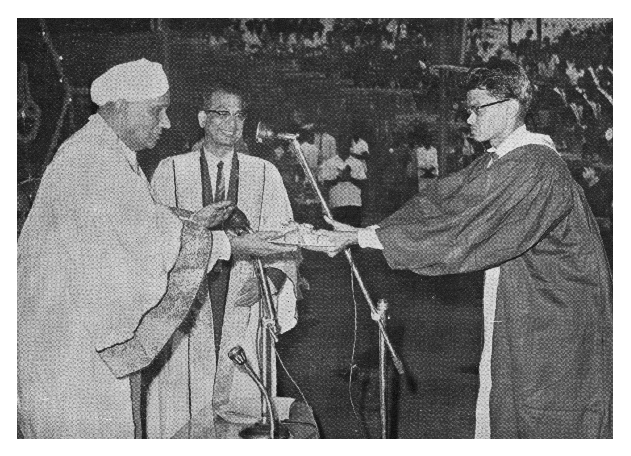
\includegraphics{eps/15.eps}

{\fontsize{10pt}{12pt}\selectfont\em Raman presenting a diploma to a student at I.I.T. Convocation.}\relax
\end{figure}

You, by the great kindness of no less than three mighty powers, the Central Government of India, the local Government of Madras, to say nothing of that mighty German Republic, have been privileged to live in this wonderful area, with these magnificent hostels, with these great laboratories and, above all, in the midst of these lovely trees and open air. You at least will not die of tuberculosis. I was privileged to be shaken by the hand by some of your prize men. I considered it a privilege to shake hands with them. If I did it with all the graduates, my hands will not be fit to hold anything. They were hefty young fellows with plenty of grip in them. That is as it ought to be. What use are you engineers if you cannot lift up a hammer? Physical strength, energy are the basis of engineering. So, I find, you have been taken care of well.}\relax
\end{quote}

\noindent
{\em The German gift}
\begin{quote}
{\fontsize{10pt}{12pt}\selectfont
It is only right and proper that I should make some reference to the great country, Germany, which has helped in no small measure to make it possible for you to receive the education that you have had during these years. To me, when Germany is mentioned, I do not think of Germany on the map. Germany brings to my mind the great masterminds which made Germany what she was. I can mention a score of names. I just mention two who have been recognised as among the greatest of philosophers and men of science the world has ever seen.
Hermann Von Helmholtz\index{Helmholtz, Hermann Von} in the 19th century and Albert Einstein\index{Einstein, Albert} in the present. I could recite a score of names. Every one of these has written his name in an imperishable way in the records of Science. These, and not the country Germany, nor all that happened to Germany, recall Germany to my mind. It was for many years my earnest desire to go round and spend a few weeks in Germany, visit these ancient centres of learning, small though they may be in geographical extent but great in the lustre of their names. Heidelberg, G\"ottingen, Marburg and so on. I will never be fortunate enough to spare that time or get that opportunity.

But ten years ago, I received an invitation to attend a conference at Lindau and I thought here was the opportunity for me. I went there, and Lindau is a curious place. How curious it was, I will not mention. It is a place on the edge of the lake we call Lake Constance, the Germans call it Bodensee, whether it is the correct pronunciation, I don't know. Lovely little place and it was a free city of the Empire. And one of the freedoms it possessed was to be allowed to run a casino, or a gambling place. You know it is not a very nice kind of freedom. They ran it and made and still make money. People think that when you go to a gambling den you are going to make money. Nothing of the sort. It is the man who keeps the gambling den who makes the money. Lindau made a substantial profit every year and the conscience of the councillors bothered them a little at having this ill-gotten wealth. So what they did was to compromise with conscience. Every year they have a Conference to which they invite nobody other than a Nobel Prize man. A Nobel Prize is the minimum qualification to be invited to this Conference. Year after year, they hold it in succession. Ten years ago, I was invited to this Conference. I went there, I was not sorry I went there, because it is a lovely place. The most beautiful place, right in the middle of the lake, is an island called the island of Mainau. Mainau is owned by Count Bernadotte. He comes from the Swedish Royal family. He was the host of this function.

\newpage

Afterwards I moved on to that old university, one of the very first universities which gave an honorary degree, the ancient University of Freiburg\index{University of Freiburg} in Breisgau. I was there for a week and then I moved on to Bonn. And then from Bonn to Munich before I came out of Germany. I am mentioning this because I was in Bonn for just a week. I had a wonderful time. You know, at that time, Germany had, even in 1956, not recovered from the devastations of the War. They were working very hard to clean up the devastation. I was enormously impressed by the Museum of Mineralogy which had been set up in Bonn. It is absolutely incredible how from a devastated country they could get together such amazing beautiful collections of rare and beautiful specimens. That is one of my happy experiences. Others I will not mention.

And on that occasion, it so happened --- all this is introductory to my remarks that when I was there, our late Prime Minister, Jawaharlal Nehru,\index{Nehru, Jawaharlal} was also there. I want you to realise that he was not there because I was there. Nor was I there because he was there. A pure accidental coincidence. Such coincidences always happen, as you know. I think the Indian Ambassador there thought that this opportunity should not be missed. So I was invited to a lunch in the President's house at which the President of the German Republic, Mr. Nehru, the Indian Ambassador and a few others sat round the table. One of the curious things that happened at that meeting was the President made a speech in German which lasted about 5 to 10 minutes. And then, at the end of it, the interpreter got up and translated word for word the whole of the 10-minute speech in English. Then Mr. Nehru got up and made a speech in English. The interpreter got up and translated the whole speech word for word into German. But I must confess that I do not remember at this distance of time what exactly they spoke. But I presume it was the usual declarations of mutual love and affection which are always made when great dignitaries meet. Why I am mentioning this is because, it was on that occasion, I read from your book, that the German Republic promised to give a gift of this Institute.

Well, just ten years ago, imagine ten years ago. I find it very difficult to understand how in the course of ten years a veritable jungle full of, presumably, snakes and cobras has been transformed into this beautiful place of learning and how so many buildings and so much equipment and so many bright young people from all over India have gathered together and such a magnificent assembly presented for my delectation. I enjoy this, particularly because I love colour. As I have mentioned on many occasions, there is an unwritten law that men should not wear bright colours as a rule. Women are allowed to wear colours as you know and they always do. But there are exceptions. And a convocation is one of these exceptions when the men are allowed to flaunt all the bright colours in the spectrum and a few outside the spectrum as well, for the delectation and admiration of those round them and specially members of the feminine sex who will be around.
}\relax
\end{quote}

\medskip
\noindent
{\em Youth and freshness of outlook}
\begin{quote}
{\fontsize{10pt}{12pt}\selectfont
Well, as I say, it is a very enjoyable occasion and I think my young friends are all extremely happy to have had this great occasion. It must stand out in their memory for a long time to come as the unique occasion in their life. Well, I remember myself, you see my mind goes back to a period sixty years ago, fully sixty years ago, I also came out of a college which is in the same town, with a degree in my pocket and a few other things, I won't mention what. Now that occasion stands out for one reason and I want to mention that reason. Looking back over the years, I find to my astonishment, to my surprise, that the experiences which I went through in those four years have left an indelible impression on my mind, an impression that sixty years of time and all that has happened since has not succeeded in dimming in the least. What is even more remarkable is this --- it is perfectly true to say that what I am today, what I have done in the last sixty years, has all been determined for me with absolute mathematical precision by what I did in those four years. The opportunities that I had during those years, made me turn my mind to certain things. I have found it impossible to turn away from these, because of the force in me of those youthful days. I was only 14 years of age when I entered the Presidency College and 18 when I came out with my Master's degree and an appointment as an Officer of the Finance Department, and a published paper as a budding scientist. All these at the age of 18! At that early age, the mind is so impressionable. And what I did then had determined my whole career.

I want to stress this because I want you, my young friends, to realise that in these years, three or four or five years as the case may be, you have been subjected to the influence of a band of teachers, you have been subjected to the influence of the old banyan trees around, which I don't regard as unimportant. Now these, please do remember that, in fact, are going to determine your future career. But that is not all. What you are going to be, my young friends, depends upon what you are going to do in the next few years to come. Alas! It is often very true that people get a degree, get a job and perhaps get married, and then forget all about what they learned in college. That is hardly the thing to do. If you are all going to be worth any little at all in the future, it can be only if you remember what has been laid now as the foundation in these four or five years. On that foundation you must build.

You always have to remember a few things, you will permit me to remind you of them. This most wonderful possession that you all have, everyone of us has, is this human body. It is our parents who gave it to us. I have recently turned my attention from physics and chemistry, mineralogy and mathematics to the study of the human faculties. Some of them, unfortunately, are hidden away inside the brain and we have to take them for granted. The mere study of all these external points of contact has made me realise what an amazing possession we have.

There is another little thing that we all forget very often. There is a little thing called the `heart'. That little machine started working when you were born, why even before you were born and goes on ticking at a certain rate and it goes on ticking, ticking, ticking all the time at the same rate, at nearly the same rate, all the time when you are young and all the time when you are getting to be an old man, until you are dead. And when that stops, you are dead. That wonderful machine, my dear young friends, has to be safeguarded. You often hear of great men suddenly dropping down, their doctors call it coronary thrombosis or whatever other names, learned names for this collapse which causes death. And why is it that this happens? It is because they over-drive this wonderful machine. They misuse their bodies. They think, now that I am so young and energetic, I can do anything I please, I can eat all the chillies I want, go out all night, attend theatres, friendship parties and so on. And what happens? No doubt the young blood can stand the strain, but it tells. And what happens then? You are prematurely aged and then coronary thrombosis comes in and takes you away. I want you to realise this at the time of youth. This is a lesson I have learned myself. Please do not think that I am preaching what I don't practice. I have always practiced it. I believe not in precept but in practice. Always, I believe that the greatest influence that a teacher has is, as they say, by his example and not by his perception only. Now is the time when you are still young, when the blood is still flowing warmly in your veins and arteries, now is the time to improve on what you learned here.

India has an enormous population. We are all trying to make India great. But who is going to make it great? It is only the young intelligentsia of the country. Realise it is up to them to use not only their hands but use their brains to learn to think. The faculty of independent thinking must be applied to all problems of life. You must be serious about life. You must not think that hasty pleasures or indulgence in all sorts of loose things are going to help you at all. This is the lesson that I have learned in these sixty years of life, actively as a man of Science. There is nothing that makes a man so happy as some real achievement. It is the achievement of doing something real that has a permanent value and will be recognized all the world over. The money bags that you find in the Reserve Bank are nothing when compared to this achievement. The mere joy of achievement is something very great. And I think all our young people who come out of our Universities realise that it is up to them to see how best they can raise the glory of India and how best they can make themselves happy, how best they can achieve even material success. It is only by realising this while they are young, while they have energy, this will be possible.

I am almost inclined to enter into a dissertation on old age versus youth. I could speak for half an hour on that thesis, `Age versus Youth'. You know that age is credited with wisdom. With all deference to the people around, I beg to question that proposition. I tell you what youth brings along with it. If you do not take care of yourself, you are left with creaky bones, your teeth drop out, your eyes become blurred, your ears become half-deaf and, worst of all, you become cynical, contemptuous of others. You come to think life is not worth living. And, in fact, you come almost to such a stage that but for the unfortunate desire we all have to continue to live, the easiest plan would be to swallow a tube of morphia and be done with it all. We do not feel like doing it and that is because God has implanted in us an absolutely unhealthy desire to continue life in spite of these miseries. I tell you that because it is very, very difficult indeed to summon up, as you grow old, those enthusiasms, those fears, desire for, achievement, energy and all that. Youth is the most glorious time of all. I have said elsewhere that most of the great discoveries in Science have been made by young people. It is not the experience or wisdom that old age brings, but the freshness of outlook, the indomitable desire to achieve, which is the characteristic of youth, that makes discoveries possible. It is this that makes life worthwhile. If only you realise this and realise that here I am, I am still young, let me see what I can do, that all discoveries become possible.
}\relax
\end{quote}

\medskip
\noindent
{\em Fearlessness and independent thinking}
\begin{quote}
{\fontsize{10pt}{12pt}\selectfont
And above all, in my own experience, I have found that one of our evils is that for centuries we have been trodden under the feet of conquerors from abroad. I don't want to recite all their names. One of the things that has been bred in us, a very deep and ineradicable defect, is a kind of inferiority complex which makes us think that we dare not question what has come to us from abroad. Whatever comes to us in a textbook must be right, some great man has said something, well, we must bow to him in fear and trembling and never question him. This produces a mental inhibition. Now, I do not suggest to you that you should all become arrogant, contemptuous of all the great men of the past. Not at all. I am not suggesting that. But I think we should all learn that no one is infallible. Not even Hermann Von Helmholtz,\index{Helmholtz, Hermann Von} not even Einstein.\index{Einstein, Albert} Nobody is infallible. New knowledge may upset what may have been made in the past, and may completely throw out what has been done before.

So I think one of the things all Indians should learn is fearless independence of thinking. That is a quality which is very essential and the absence of which, if I may venture to say so with all deference, is what stands today in the path of Indian progress. Whenever we want to do anything, we borrow money from abroad. We all know that every day we see one hundred million dollars or one billion dollars being borrowed from somewhere. Our so-called independence freely consists, if I may say so without entering into politics, in our being ruled by a consortium of all the nations in the world, except ourselves. Leave that alone. Bad enough to borrow money. But what about borrowing knowledge? What about borrowing experts from abroad? What about forgetting to think for ourselves? This feeling of helplessness must be shaken away, shaken out ruthlessly. We must realise that we must stand on our own legs. It is better to work with the most inefficient useless equipment of ours than to shine in borrowed feathers, better to work on problems with our slender resources. We must realise this and until and unless we realise this, we cannot go on. And I want to turn to my great industrialist friends who want to buy know-how at great expense from abroad. Let me assure them that they will never get on and get very far. You see that the signs are already there. The rupee has come down, I do not know to how many cents, and Mr. Masani\index{Masani} has said that it will soon come down to five cents. I am not wishing that his prophesy comes true.
}\relax
\end{quote}

\noindent
{\em Science and Technology progress}
\begin{quote}
{\fontsize{10pt}{12pt}\selectfont
But no country, and as you are all engineers, let me express here forcibly my conviction that no country can become industrially great without a foundation of real knowledge. This is what Science teaches. Science has shown time and again that Science comes first and Technology afterwards. Without Science, there is no Technology. Why has Germany been so great? Because in the 19th century, she had a galaxy of men of Science in every branch of knowledge, whose name and fame shone forth. Because they were not technicians, they were humble professors in the universities. But they sought knowledge and they made their students seek knowledge. They were springs from which knowledge came forth, gushed forth and it was that knowledge, that spring of knowledge, that fertilised all the industries of Germany and made her great.

It is realised in all countries today, that Science comes first and Technology afterwards. If you think you can build a great industrial nation, make tons of money and pay off all these awful debts by pursuing so-called Technology alone, you are doomed to complete failure. Let me say this without hesitation. It is only when we set our houses in order and build up powerful schools of thinking in every field, electricity, chemistry, metallurgy and so on, only then we will have the solid basis of knowledge from which can come forth men who will teach your technologists what to do. I think it is true to say that the finest instruments, the most sophisticated instruments, are not found in technological laboratories, but are found in the research laboratories where men are trying to explore the unknown world and try to discover things. There is also another thing which is well worth remarking upon and that is, in not a few cases, not only is Science the fountain-head of technological knowledge. In many cases Science has set the problems which the technologists had to solve.

You may recall the history of Astronomy of the 19th century. Astronomy is usually regarded as one of the useless subjects. Our ancients were much concerned about the stars because they thought that the sun and the stars had something to do with human affairs. So they very keenly watched the planets and the stars. Though the reasons they may have done so may be wrong, there is no doubt that the pursuit of astronomy is of infinite importance to us. The study of astronomy may look as if it has nothing to do with human affairs, if you do not believe in astrology, but really it is more from the study of the stars that you have learned more about the earth we live in, more about the Sun and more about everything, than from the study of terrestrial sources of light. The astronomers demanded instruments of the highest precision with which alone they could follow the movement of the stars, do the time-keeping, note the displacements, aberrations. parallax and so on. The demands of precision instruments, especially by Germans like Bessel and others, led to the modern development of precision mechanics. You understand what I mean by precision mechanics. I wish to mention the fact that the great telescope at Palomar, the 200-inch telescope, that enormous thing, that tremendous, huge, massive thing, hundreds of tons in weight, has to be moved with the accuracy and precision of a Swiss watch and nothing less. Nothing less will satisfy the astronomers. This huge mass has to go round with the smoothness and precision of a Swiss watch. I know what the precision of a Swiss watch is. I have got here a watch on my wrist which I wear only on occasions such as this. Well, I want to be reminded of the time which passes and I wind it only about once a year or so. But all the time it shows the correct time. Astronomy demands such precision and it was the demand of the astronomers that led to the development of precision mechanics which, of course, today we use in everything.

You can quote example after example to prove this. The demands of Science, the botanist, the zoologist who wanted to examine his subtle structures led to the development of the great firm of Carl Zeiss. It was Ernst Abbe\index{Abbe, Ernst} who took up that problem and made the optical industry what it is today. What was demanded and made for the needs of Science has benefitted everybody else. The same story is repeated in all the beautiful instruments that have gone to make this great advancements of knowledge possible in these sixty years. They were born out of the brain of men of Science, they were translated into practice and today they are the tools of study in every branch of knowledge. Every metallurgist today uses the electron microscope. Who thought of it? A man of Science who was not interested in its possible applications. He was interested in it for its own sake.

Now I wind up. I think I have gone on long enough. I must stop. I know you are all listening to me with great eagerness and interest. I must put an end to your agonies. I will do so as soon as I can. But this I would like to say, that the developmemt of knowledge and Science in the last sixty years, I have seen from the inside. I have not been inside all the time, but I have been inside most of the time. It has been something absolutely fantastic.
}\relax
\end{quote}

\medskip
\noindent
{\em The nature of scientific advances}
\begin{quote}
{\fontsize{10pt}{11.7pt}\selectfont
Why is it that Science has developed in such an explosive or spectacular fashion in the last sixty years? There are really three causes. We can analyse them and put them apart. First and foremost stands the fact that towards the end of the 19th century, or in the beginning of this century, came a succession of epoch-making discoveries in fundamental knowledge, the discovery of the quantum of action by Planck,\index{Planck, Max} the discovery of Einstein\index{Einstein, Albert} of the corpuscular nature of light and then the use of this principle by Neils Bohr\index{Bohr, Niels} and others to analyse the structure of the atom, to explore the chemical molecule. This sort of explosive development at the beginning of the century made a terrific advance possible, in the study of the ultimate structure of matter, and this explosion is still going on.

There is a second and a great stream of scientific knowledge which has come out in this way. And that is the fact that Science, as we all know and recognise it, has very definite applications to human welfare. This is most evident from examples in the field of agriculture, the knowledge of heredity, the Laws of Mendelism and so on. They made a great difference to the science of agriculture. So also, one of the most important advances which has a bearing on the work of you gentlemen is the discovery of what is known as plastics. The whole science of micro-electro chemistry as it is called has developed from the work of a man who was interested simply in studying the big molecules, Staudinger.\index{Staudinger} Then the subject took on an explosive development. Today we can't live without plastics. We drink our coffee out of plastic cups. We wear artificial silks made of nylon and plastics. It is a typical example of how pure Science has led to the development of vast industries with the greatest possible importance. Then we have also examples in medicine. From ancient times, the human body has been subjected to all kinds of illnesses and the `medicine men' with their drugs did a roaring practice. The modern expression with regard to those funny people calls them `witch doctors'. From the medicines of these witch doctors to the modern medicines, the leap has been marvellous.

But there is a third and a most sinister way in which Science has developed in the last sixty years. And that is Science in its applications to war, application to defensive war and offensive war. Even in medicine, much of our knowledge of the human brain has come from the study of half-dead and half-dying men in war. The examination of their bodies has led to a profound advance in medical knowledge. So war has had that result. I think we can say that a lot of modern Science has really come directly out of the needs of war. I knew for example, in the First World War, men like Lord Rutherford,\index{Rutherford} Sir William Bragg\index{Bragg, William} and many other British scientists were all busy trying to combat the submarine menace by the invention of the subsonic devices that, today, are being used everywhere. Even in the First World War, the use of aviation in warfare was already being developed; in the Second World War it took a tremendous turn.}

{\fontsize{10pt}{12}\selectfont And not only that, the Second World War, as you all know, brought the atom bomb into existence. That atom bomb has come directly out of the consequence of the actual discovery of fission made by Joliot Curie\index{Curie, Joliot} in the laboratory --- he showed it to me when I was there in Paris, the gist of the discoveries made. That immediately set thinking minds in action --- here is an instrument of dreadful power, if we use it we can destroy mankind. And fear, the fear that the other man may use it led to the development of the atom bomb everywhere. Then the hydrogen bomb came. And ever since, an atmosphere of fear, it is a horrible thing to see, an atmosphere of fear of mutual recrimination, progressive deterioration is there, like what happens to a man when he borrows money. You see the interest goes on adding up. It becomes a colossal figure, which bears no resemblance whatsoever to the loan which he took at first. This kind of explosive development of fear complex has produced a psychological, a pathological state of affairs in the human mind in which all evils thrive and sustain. Today, Science in many countries is simply the hand-maid of the war machine.

Wonderful achievements, rockets sent up and two men jumped out of it and had a rope tied to their bellies and they walked in space. And everybody says: `Oh! What a great feat!' Let me tell you, I simply smile with loathing and contempt. It is with feelings of loathing and contempt with which I witness this colossal display of lunacy on the part of mankind. It is nothing less than lunacy, sheer raving lunacy, to spend billions of dollars. Instead of shooting two men into space they could have shot two monkeys and made them walk in space. It is just a mere pretence. I say this with all sense of responsibility, it is a mere pretense to say that all these exploits of finding out what exactly is there on the moon and so on, have any scientific value whatever. I absolutely deny that. It is nothing but militarism very thinly disguised. That is what is happening today. It is very sad. Our Science is going that way. So Science today is misused.

I heard the pledge given by you, that you will not use your knowledge for unworthy ends. If you had been in one of those countries you would have to use it for unworthy ends. Otherwise you would lose your job forthwith. What is the use of giving a pledge which you would have to break in order to get your daily bread? This is what is happening today. There are sensitive consciences even in those countries who revolt from this sort of thing. But it is going on, going on, this prostitution of Science. Where it will end, I do not know.

Only I want to say this, that we in India to some extent are slaves. We are part of the machinations of our so-called friends. We are forced to accept this situation. Our friends in the United States give all the latest arms to our friends in Pakistan and they want them to use these against us and they have used these against us and we are forced to reply in time. The Russians thought that the Chinese were a friendly nation. They taught Chinese all the arts of war. What China is doing today is what Russia had taught her to do, and now China is paying her back in her own coin. This is a horrible situation. I do not know what to do. As a man of Science, my heart is simply wrung with this amazing prostitution of Science. We can do nothing about it. In fact, we have to accept the situation as it is and do what we can. I am sorry to have had to end on this very unfortunate and depressing note. There it is.
}\relax
\end{quote}

\medskip
\noindent
{\em Self-reliance, the need of the hour}
\begin{quote}
{\fontsize{10pt}{12pt}\selectfont
But let me end by saying that we in this country have no future whatever of any sort unless we learn firstly, secondly and lastly to rely on ourselves for everything that we need. It is better, I think, to go back to the Gandhian age and ride an ox-cart, to throw away radio, television and everything and go back to the land of the ox-cart. We cannot do it unfortunately. We are tied to the coat-tails of European civilisation, I include myself also in this. In the first place I put a big query mark after the word `civilisation' and I must also put another mark after `European'. I must also add American, you know the American way of civilisation. We are tied to their coat-tails. We find that we cannot be happy unless we have a radio making a lot of noise in the other room. I never listen to a radio. I simply loathe it. One of the things that we have been taught from childhood is to admire this wonderful flicker on the screen. I never go to a cinema, never. For twenty years I have not stepped inside a cinema theatre. I cannot advise my young friends to follow my example because I know they won't follow my example. We are told that we cannot be happy unless we have a television set to see some lady dancing on the television screen. This is the trouble.

You see our tastes have been corrupted. We do not want to look at the banyan trees. We must go and see the cinema screen. Now we must, I say this with all energy that I can command, we have to eschew all the evil things whlch we learn from Europe and America. Let us not condemn Science for that reason, but we must not subordinate ourselves to the ideas and ideals which have come to us from the West, which are simply designed to make us part with our rupees and make the rupee worth five cents, as Mr. Masani\index{Masani} says.

If we cannot do these things ourselves, let us do without them, as I say, let us walk, let us go in the country carts. If we cannot make our motor cars, why should we buy them from abroad? Why even import parts? It is one of those funny things, it is said ``Oh! 85 per cent is `local made' and the remaining 15 per cent is imported". They talk of electronics. I have tried hard to find out if there is any one place --- I have not yet heard an answer to that --- if there is any place in India where the most important component of all electronic valves is made. All these depend upon the manufacture of a metallic filament which will stand the current. If they are being made in India I should like to know where they have been made. I have not heard of any. That is the starting point of the whole electronic industry and do we make it? Let us wait till we can make it, before we buy a single electronic valve from outside. If we do that, then I think we would learn, how to make it. It is this lesson of self-reliance that we have to learn and until we learn it there is no future for us."
}\relax
\end{quote}

This address, spoken from the heart, defines Raman's views on a wide range of topics and issues. No one in India of his stature expressed his views so fearlessly as Raman did.

Intensely national, Raman spoke in no uncertain terms of his abiding faith in the younger generation and this made him feel not so desperate about the `brain drain' as others. The proper attitude of Science and scientific research was to him more important than fancy laboratories. Once he remarked, ``The essence of Science is independent thinking, hard work and not equipment. When I got my Nobel Prize, I had hardly spent Rs. 200 on my equipment. See my `Physiology of Vision' research. All the equipment with which I worked for this book is here in my table drawer, devised by me". On the occasion of the opening of a laboratory he asked cryptically: ``Where are the brains to put into this magnificent building? Remember, Radium was discovered in a tin-shed!"
\index{Indian Institute of Technology Convocation Address|)}

\medskip
\heading{Raman's contributions to Science in India}
\addtocontents{toc}{\protect\contentsline{section}{Raman's contributions to Science in India}{\thepage}}
\smallskip

\index{Raman, Chandrasekhara Venkata!Papers/Publications/Addresses}

\lhead[{\it\fontsize{9pt}{9pt}\selectfont\thepage}]{\it{\fontsize{9pt}{11pt}\selectfont Raman's contributions to Science in India}}

\noindent
Raman was a great builder of institutions and centres of research. He revived and revitalised the Indian Association for Cultivation of Science\index{The Indian Association for Cultivation of Science} and established the Departments of Phy\-sics at the University College of Science in Calcutta and at the Indian Institute of Science,\index{Indian Institute of Science} Bangalore, and founded the Raman Research Institute,\index{Raman Research Institute} making them all centres of world renown. He recognised the importance of scientific journals and started one in Calcutta under the Indian Association for Cultivation of Science, which later became the {\em Indian Journal of Physics}.\index{Indian Journal of Physics} When he moved to Bangalore, he founded another journal called the {\em Proceedings of the Indian Academy of Sciences}.\index{Proceedings of the Indian Academy of Sciences@\textit{Proceedings of the Indian Academy of Sciences}} He was also actively involved in the starting of {\em Current Science}\index{Current Science@\textit{Current Science}} in 1932, which was styled after {\em Nature}.\index{Nature@\textit{Nature}} He believed strongly that the best work done in India should be published in Indian journals, and set a personal example by publishing all his papers in the journals he started. Raman's, as well as the work of his students, fill the pages of the {\em Proceedings of the Indian Academy of Sciences}.

\vskip .1cm

Recognising that a scientific forum was necessary to bring awareness of Science to the layman and to the Government, he founded in 1934 the Indian Academy of Sciences,\index{Indian Academy of Sciences} to which outstanding scientists from all over India were elected as Fellows. The {\em Proceedings} that issued from the Academy and its annual meetings were regular features. Raman was elected its founder President and he held the office until his death in 1970. He also served as the editor for the {\em Proceedings} and set the highest standards for the journal. The {\em Proceedings} came out promptly every month in two sections, A and B, for physical and biological sciences respectively, and were dispatched to all the subscribers in India and abroad. The {\em Proceedings} of the Academy were considered as being among the top journals of the world.

\vskip .1cm

The lofty ideals with which the Indian Academy of Sciences was started and the {\em service to the nation} which it was expected to \hbox{render} were eloquently described by Raman himself at its first annual meeting in Bombay. On that occasion he said:
\begin{quote}
{\fontsize{10pt}{12pt}\selectfont
``I think it would be not inopportune to consider at this stage the nature of the services which the Academy can render to Science in India. We live in an era of scientific progress and it is a very gratifying feature that India is beginning to pull its weight in this respect. Modern scientific progress shows side by side two apparently contradictory features. On the one hand, we have an enormous accumulation of raw scientific material, the significance of which, in many cases, is hardly apparent except to specialists in very limited fields of investigation. On the other hand, we have a great process of scientific synthesis going on, tending towards the simplification and unification of the fundamental principles of natural knowledge in all its ramifications. It should never be over-looked that Science is in reality a great impartible estate and that the boundaries drawn across it to divide it into restricted fields are in essence artificial. I think the history of Science has shown over and over again, that it is only by boldly cutting across these artificial boundaries that progress of real significance can be achieved. It is precisely this feature that lends importance to the activities of such an Academy as ours, where men of Science of widely different scientific interests come together in a common endeavour and seek to understand each other's point of view.

While specialisation is necessary, an excessive narrow outlook defeats the primary purpose of Science, which is to advance our essential comprehension of nature as a whole. It is, therefore, one of the most important functions of our Academy to promote co-operation between men who profess knowledge of different branches of Science. This is effected in various ways. In the {\em Proceedings of the Academy},\index{Proceedings of the Indian Academy of Sciences@\textit{Proceedings of the Indian Academy of Sciences}} the Fellows and, indeed, all scientific men have an opportunity of obtaining at least a general idea of what is being done in India in fields of knowledge other than their own specialty. In the scientific meetings of the Academy and especially in the symposia they have a valuable opportunity of discussing problems of common interest from different points of view.

I will also say a word about the Academy, in relation to the nation at large. It is inevitable that the Academy, consisting as it does of the most active workers in the country who are representatives of the \hbox{different} parts of India and of different branches of Science, will soon come to be regarded as the most authoritative body to speak in the name of India on all matters touching the progress of Science. The potentialities of such an Academy in the way of national service are almost unlimited. What it can actually achieve depends on the measure of support it receives from the Government of India and from the general public. I do not think that any calls for service from responsible quarters will find us unwilling or unprepared."
}\relax
\end{quote}

With the passing away of Professor Raman, the Indian Academy of Sciences\index{Indian Academy of Sciences} and its {\em Proceedings} with their well-establi\-shed scientific traditions, have passed into the hands of other Indian scientists as two of his most valuable legacies to them.

Raman took a personal interest in all the affairs of the Academy; publication, meetings, elections and actual running of the organisation. He had the trusted and loyal assistance of B. S. Venkatachar\index{Venkatachar, B.S.} in managing the day-to-day affairs of the Academy. The Academy office was located in the Raman Institute campus and Raman would walk to the office almost every day to discuss matters concerning the Academy with Venkatachar. The principal activity of the Academy was the publication of its journal, the {\em Proceedings}. Most of the papers published in the {\em Proceedings} were scrutinised by Raman himself for scientific merit, importance and presentation. He was very particular that the journals were brought out promptly at the end of each month and mailed to the Fellows and subscribers on the first of every month.

Raman took a very keen interest in the election of Fellows to the Academy and, in those days, the number of Fellows elected would, at the most, be half a dozen. Raman personally looked into the nominations and discussed the merits of the candidates at the Council meetings which usually made the recommendations to the General Body. Raman himself proposed candidates if he felt that the persons concerned were active research scientists showing promise for the future. 

\newpage

One fine morning in 1954, he came to me and said, ``I am proposing you for election as a Fellow of the Indian Academy of Sciences''. I was taken aback and told him, ``Sir, how do I deserve such an honour at this point?'' His reply was, ``I know how to judge people and when to honour them and encourage them. I don't recommend anyone who does not deserve the honour''. I was elected that December as a Fellow of the Indian Academy of Sciences.

In 1956, the Treasurership of the Academy fell vacant and, at Raman's suggestion, I was installed as the Treasurer, in which capacity I served until I left Bangalore. By virtue of this office I was also a member of the Council of the Indian Academy of Sciences, which shaped the policies and activities of the Academy under the stewardship of its President, C. V. Raman. During my tenure I had the pleasure of sitting with some of the finest people in the scientific field in India, including S. Bhagavantam,\index{Bhagavantam, S.} who was at that time Director of the Indian Institute of Science, M. V. Govindaswamy,\index{Govindaswamy, M. V.} Director of the Bangalore mental health hospital and who himself was a clinical psychiatrist, B. S. Madhava Rao,\index{Madhava Rao, B.S.} Principal and Professor of Mathematics at Central College, Bangalore, B. K. Narayana Rao,\index{Narayana Rao, B.K.} a well-known opthalmic specialist in Bangalore, C. S. Pichamuthu,\index{Pichamuthu, C.S.} Director of the Mysore Geological Survey, and L. Rama Rau, a paleontologist and retired Professor from Central College.

Raman presided over the Council meetings and it was a pleasure as well as a great experience to hear him at these sessions. He would, of course, dominate the floor at the meetings which were attended by half a dozen Councillors. Good  tiffin and excellent coffee were served and relished by everyone at these very enjoyable meetings. Raman got whatever he wanted from the Council and the meetings always ended on a happy note. At one of these meetings, Narayana Rao, made the suggestion to Raman that younger people should be brought into the Council. I remember very well Raman's remarks. ``Dr. Narayana Rao,\index{Narayana Rao} nothing like old shoes. They are very comfortable and do not bite your toes and cause you trouble. I prefer wizened, grey and mature heads, preferably wearing a turban." Both Raman and Narayana Rao wore turbans. Everyone had a good laugh.

Raman organised the annual meetings of the Academy meticulously, with scientific programmes and public lectures. The best work done by the Fellows and their associates were presented at these meetings at which Raman's public lectures were usually the high points. The Academy met at the invitation of a University serving as the host, so that young students of Science got exposed to the scientific body and heard India's foremost scientists in person.

\vskip .1cm

I attended ten of these meetings. Raman would sit through all the sessions, covering both physical and biological sciences, and added lustre and humour to the proceedings. He would ask the most penetrating questions and make very entertaining comments. It was dangerous to give a talk before him that had no originality, for he called spade a spade right in front of everyone. These annual meetings were jocularly referred to as ``Raman's circus". He never failed to be present at these meetings, except once towards the end of his life. The Indian Academy of Sciences\index{Indian Academy of Sciences} has redoubled its activity and its publication efforts have multiplied several-fold in the post-Raman era.

\vskip .1cm

In assessing Raman's place in Indian Science, the following quote from a jubilee volume which was published in 1938, to felicitate him on his 50th birthday, might be considered a pointer. At that time, he was practically at the peak of his scientific fame, having achieved his ambition of creating a strong school of modern Science in India.
\begin{quote}
{\fontsize{10pt}{12pt}\selectfont
``He is the outstanding figure in the renaissance of Science which has been taking place in India during the last quarter of a century, and indeed with truth he may be designated as the creator and leader of that renaissance. The progressive enthusiasm for scientific studies and research which is witnessed on all sides in India today has largely been inspired by him and encouraged and sustained by his efforts.

The personal example of his dedication to a scientific career, the brilliance and originality of his researches, the international character of the recognition which his work has received, his success as a teacher in training investigators who are now themselves guiding schools of research, his gift of eloquence which has served to stimulate a\break \hbox{wide\-spread} interest in Science, his achievements as a scientific administrator in creating facilities for research and establishing new schools of Science, and his success in founding journals for publication of scientific work in India, are among the factors which have profoundly influenced the progress of Science in the country."}\relax
\end{quote}

This Summary in 1938 about Raman's contributions to Indian Science proved even truer in the years that followed.

\vskip .1cm

Towards the end, Raman\index{Raman, Chandrasekhara Venkata!Traits/Interests} turned somewhat bitter and cynical ab\-out politics in Indian Science and scientific development in the country. He shunned all the activities of present-day scientists in India. He did not believe in big scientific organisations and was suspicious of scientific administrators. He used to say, ``For such people, the so-called organisation of Science becomes more important than Science itself, or its values". But to the very end he never gave up his interest in pursuing his own scientific activity or of trying to arrange for the future of his Institute after him.

\vskip .1cm

Prof. Ramaseshan, his nephew, who was at the National Aeronautical Laboratory in Bangalore, became quite close to him during his last few years and Raman often discussed the future of the Raman Institute\index{Raman Research Institute} with him. After Raman's death it was his wish that the Directorship of the Institute be offered to his son, Radhakrishnan,\index{Radhakrishnan, V.} a well-known Radio Astronomer. Ramaseshan took a very active role in carrying out Raman's wishes.

\vskip .1cm

Raman was a staunch nationalist and was proud of his Indian heritage and its past achievements. He admired Mahatma Gandhi\index{Gandhi, Mahatma} and Jawaharlal Nehru, although he did not agree with all their policies. In the matter of scientific research, he insisted that Indian scientists should not be camp-followers and imitate what was being done in the West. He often proclaimed that what one did should not only be original but should also be relevant to India's needs when it came to application of research. He was opposed to Indian scientists going abroad for advanced research and believed that it impeded originality of thinking. It is difficult to say whether he was right or wrong, but it is a fact that independent India is yet to produce scientists of Raman's calibre, although the money spent on scientific research is enormous compared to the Raman days. Raman may have had a point.

\vskip .1cm

Raman was a man of emotion and could get violently angry. But he had an incredible sense of humour and could keep an audience roaring with laughter merely describing what would have been a common place incident. Above all, he was a very simple man, quite childlike, sometimes even childish. There was a condolence meeting in Bangalore when Einstein\index{Einstein, Albert} died. When Raman got up to speak, he was choked with emotion and sobbed like a child before he could talk.

\vskip .1cm

Anyone who met him could not but be struck by his zest for life. His exuberance was infectious. Chatting with him for some time was like taking a tonic. To him, scientific activity was the fulfilment of an inner need. His approach to Science was one of passion, curiosity and simplicity. Science was to him a personal endeavour, an aesthetic pursuit and, above all, a joyous experience.

\vskip .06cm

No single person has done so much for Indian Science as Raman. Through personal example of the highest dedication to Science, through his success as a teacher-cum-leader in training generations of physicists who in turn have created independent schools of research, through creating scientific institutions and facilities for research and founding scientific academies and journals for the dissemination and propagation of Science, and through his gift of eloquence which served to inspire and stimulate a widespread interest in Science, Raman, as a single individual, tremendously influenced the progress of Science in India.

\vskip .06cm

He was one of a rare breed of men who are no more, who ranged freely in all fields of science from physics to chemistry to biology. Raman stands alone as the greatest scientist that India gave the world. The poet Valmiki, describing the battle between Rama and Ravana, said in the great epic, the {\em Ramayana}, ``The sky is comparable only to the sky, the ocean only to the ocean and the battle between Rama and Ravana only to the Rama Ravana {\em yuddham} (battle)''. In modern India, Raman is only comparable only to Raman.
